\documentclass{beamer}
\usetheme{default}
\usecolortheme{seahorse}
\usefonttheme{serif}
\usepackage{amsmath, amssymb, physics, bm}
\usepackage{graphicx}
\usepackage{tikz}
\usetikzlibrary{arrows.meta, positioning, shapes.geometric, calc, decorations.markings, fit}
\usepackage{xcolor}
\usepackage{booktabs}
\usepackage[font=small,labelfont=bf]{caption}

% ─── Color palette: deep navy + gold accent ───────────────────────────────────
\definecolor{navydark}{HTML}{0D1B2A}
\definecolor{navymid}{HTML}{1B3A5C}
\definecolor{gold}{HTML}{C9A84C}
\definecolor{lightgray}{HTML}{F0F2F5}
\definecolor{mutedtext}{HTML}{6B7A8D}

\setbeamercolor{frametitle}{fg=white, bg=navydark}
\setbeamercolor{title}{fg=white}
\setbeamercolor{author}{fg=gold}
\setbeamercolor{institute}{fg=lightgray}
\setbeamercolor{date}{fg=lightgray}
\setbeamercolor{background canvas}{bg=white}
\setbeamercolor{normal text}{fg=navydark}
\setbeamercolor{structure}{fg=navymid}
\setbeamercolor{block title}{fg=white, bg=navymid}
\setbeamercolor{block body}{fg=navydark, bg=white}
\setbeamercolor{itemize item}{fg=gold}
\setbeamercolor{itemize subitem}{fg=mutedtext}

\setbeamertemplate{navigation symbols}{}
\setbeamertemplate{footline}{
  \leavevmode
  \hbox{%
    \begin{beamercolorbox}[wd=.6\paperwidth,ht=2.5ex,dp=1ex,left,leftskip=1em]{normal text}%
      \tiny\color{mutedtext}\insertshorttitle
    \end{beamercolorbox}%
    \begin{beamercolorbox}[wd=.4\paperwidth,ht=2.5ex,dp=1ex,right,rightskip=1em]{normal text}%
      \tiny\color{mutedtext}\insertframenumber\,/\,\inserttotalframenumber
  \end{beamercolorbox}}%
  \vskip0pt%
}

\setbeamertemplate{frametitle}{
  \vspace{0.2em}
  \begin{beamercolorbox}[wd=\paperwidth,center,ht=3.4ex,dp=1.2ex]{frametitle}
    {\Large\bfseries\insertframetitle}
  \end{beamercolorbox}
  \vspace{0.2em}
}

\setlength\parindent{0pt}
\graphicspath{{img/}}

% ─── Placeholder (used ONLY where no suitable image exists yet) ───────────────
\newcommand{\figplaceholder}[2][0.85\textwidth]{%
  \begin{center}
    \fbox{
      \begin{minipage}{#1}
        \vspace{1.5cm}
        \centering
        \color{mutedtext}\small\textit{[Figure: #2]}
        \vspace{1.5cm}
    \end{minipage}}
  \end{center}
}

\newcommand{\figplaceholderH}[3][0.85\textwidth]{%
  \begin{center}
    \fbox{
      \begin{minipage}{#1}
        \vspace{#3}
        \centering
        \color{mutedtext}\small\textit{[Figure: #2]}
        \vspace{#3}
    \end{minipage}}
  \end{center}
}

% ─── Title info ───────────────────────────────────────────────────────────────
\title[ConcreteNet: GPR Rebar \& Defect Detection]
{ConcreteNet}
\author{Anish Goyal, Julieta Sanchez}
\institute{Georgia Southern University}
\date{April 23, 2026}

\begin{document}

% ═════════════════════════════════════════════════════════════════════════════
% TITLE
% ═════════════════════════════════════════════════════════════════════════════
{
  \begin{frame}[plain]
    \vspace{0.2cm}
    \centering
    {\LARGE\color{navydark}\textbf{ConcreteNet}}\\[0.3em]
    {\small\color{navymid} Adaptive image-based classification of concrete rebars and defects in ground-penetrating radargrams}\\[1.0em]

    {\color{navydark}Anish Goyal, Julieta Sanchez}\\[0.15em]
    {\small\color{mutedtext} Faculty Mentor: Dr.\ Hossein Taheri}\\[0.15em]
    {\small\color{mutedtext} Dept.\ of Electrical \& Computer Engineering \\ Georgia Southern University}\\[1.0em]

    {\centering\raisebox{0.4cm}{
\includegraphics[height=1.2cm]{misc/Georgia_Southern_University_Logo.png}}\hspace{1.2em}
\includegraphics[height=2cm]{misc/image1.png}\par}

    \vspace{0.7em}
    {\small\color{mutedtext} GS4 Research Symposium \textbullet\ April 23, 2026}
  \end{frame}
}

% ═════════════════════════════════════════════════════════════════════════════
% BACKGROUND
% ═════════════════════════════════════════════════════════════════════════════
\begin{frame}[plain]
  \vspace{2.8cm}\centering
  {\Huge\color{navydark}\textbf{Background}}\\[0.5em]
  {\color{navymid} Concrete, defects, and ground-penetrating radar}
\end{frame}

\begin{frame}{Inside a Reinforced Concrete Slab}
  \begin{columns}[c]
    \begin{column}{0.5\textwidth}\centering
\includegraphics[width=0.95\textwidth]{misc/image15.png}\\{\footnotesize\color{mutedtext}Rebar grid before the pour}\end{column}
    \begin{column}{0.5\textwidth}\centering
\includegraphics[width=0.95\textwidth]{misc/image21.png}\\{\footnotesize\color{mutedtext}Corroded rebar after years of service}\end{column}
  \end{columns}
\end{frame}

% ═════════════════════════════════════════════════════════════════════════════
% DEFECTS
% ═════════════════════════════════════════════════════════════════════════════
\begin{frame}{Defects of Interest}
  \begin{columns}[c]
    \begin{column}{0.5\textwidth}\centering
      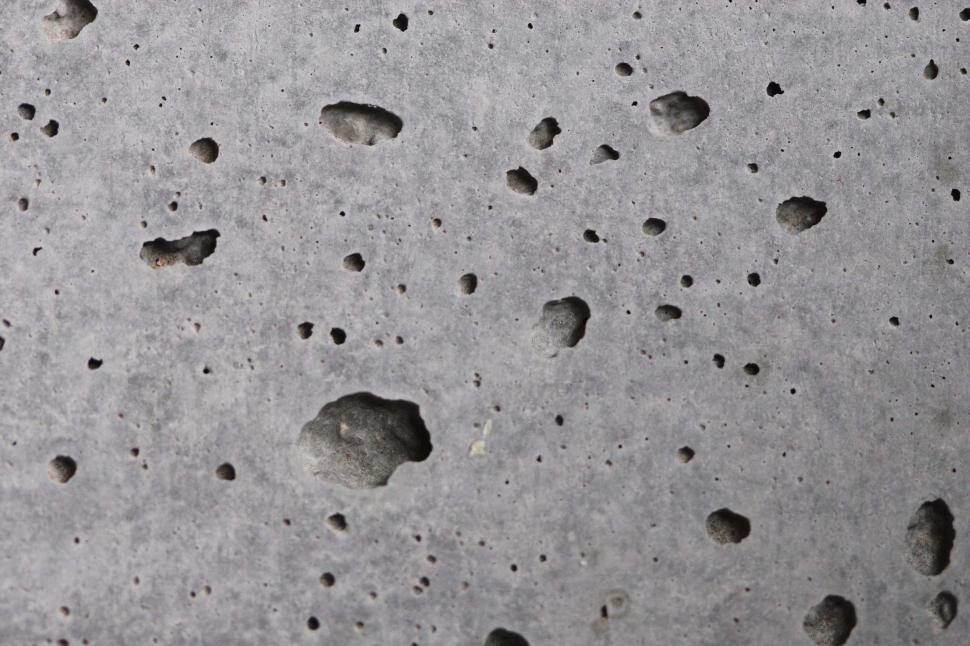
\includegraphics[width=0.9\textwidth,height=3.2cm,keepaspectratio]{defects/defect_voids.png}\\
      {\footnotesize\textbf{Voids}}
    \end{column}
    \begin{column}{0.5\textwidth}\centering
      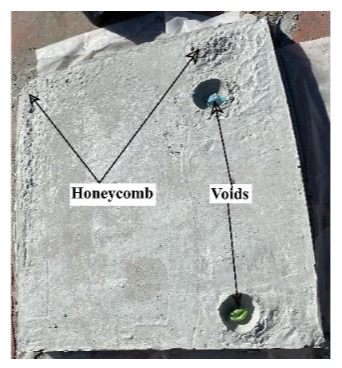
\includegraphics[width=0.9\textwidth,height=3.2cm,keepaspectratio]{defects/defect_honeycomb.png}\\
      {\footnotesize\textbf{Honeycombing}}
    \end{column}
  \end{columns}
  \vspace{0.4em}
  \begin{columns}[c]
    \begin{column}{0.5\textwidth}\centering
      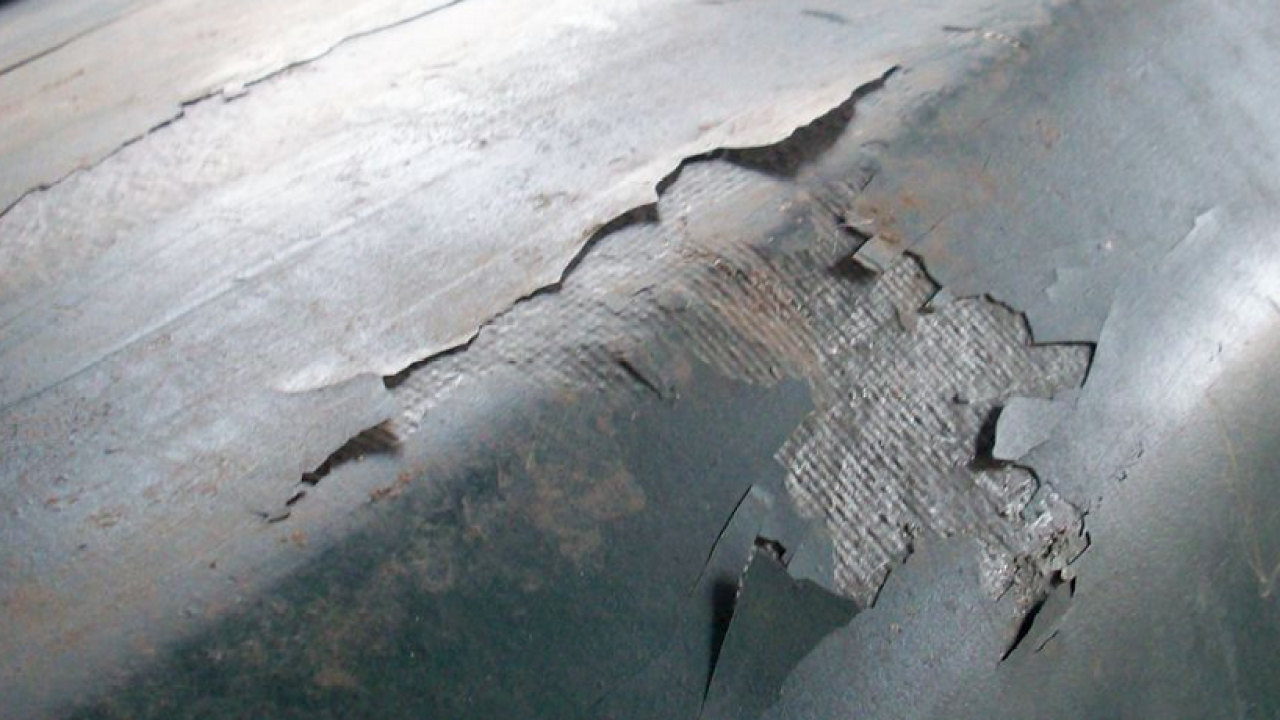
\includegraphics[width=0.9\textwidth,height=3.2cm,keepaspectratio]{defects/defect_spalling.png}\\
      {\footnotesize\textbf{Delamination}}
    \end{column}
    \begin{column}{0.5\textwidth}\centering
      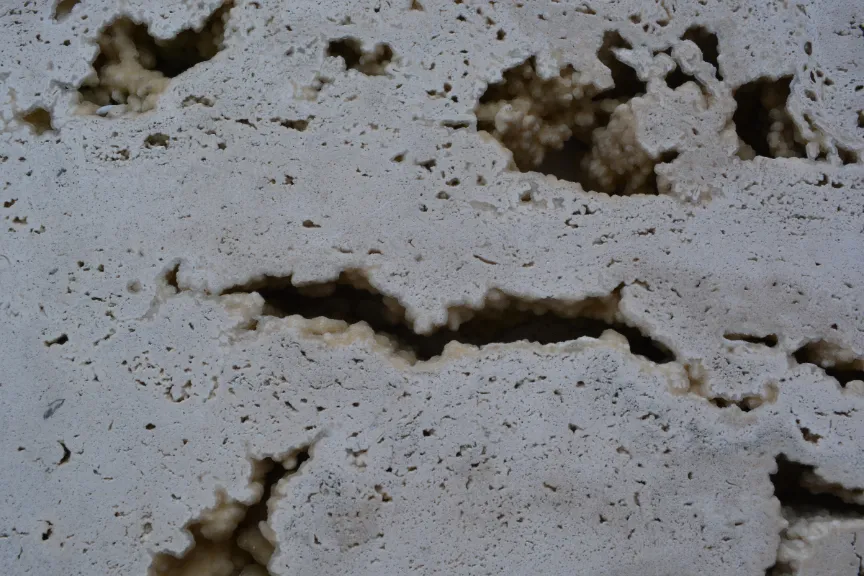
\includegraphics[width=0.9\textwidth,height=3.2cm,keepaspectratio]{defects/defect_cracking.png}\\
      {\footnotesize\textbf{Surface cracking}}
    \end{column}
  \end{columns}
\end{frame}

% ═════════════════════════════════════════════════════════════════════════════
% DESTRUCTIVE TESTING
% ═════════════════════════════════════════════════════════════════════════════
\begin{frame}{Destructive Testing}
  \centering
  
\includegraphics[width=0.78\textwidth]{misc/image22.png}
\end{frame}

\begin{frame}{The Problem With Coring}
  \centering
  
\includegraphics[width=0.58\textwidth]{misc/image12.png}\\[0.3em]
  {\footnotesize\color{mutedtext}Every sample weakens the structure you're inspecting}
\end{frame}

% ═════════════════════════════════════════════════════════════════════════════
% NDT
% ═════════════════════════════════════════════════════════════════════════════
\begin{frame}{Non-Destructive Testing}
  \centering
  
\includegraphics[width=0.72\textwidth]{misc/image19.png}
\end{frame}

% ═════════════════════════════════════════════════════════════════════════════
% GPR PHYSICS
% ═════════════════════════════════════════════════════════════════════════════
\begin{frame}{Ground-Penetrating Radar}
  \centering
  
\includegraphics[width=0.78\textwidth]{misc/image25.png}\\[0.3em]
  {\footnotesize\color{mutedtext}Antenna fires EM pulse; reflections return at each dielectric boundary}
\end{frame}

\begin{frame}{Visualization}
  \centering
  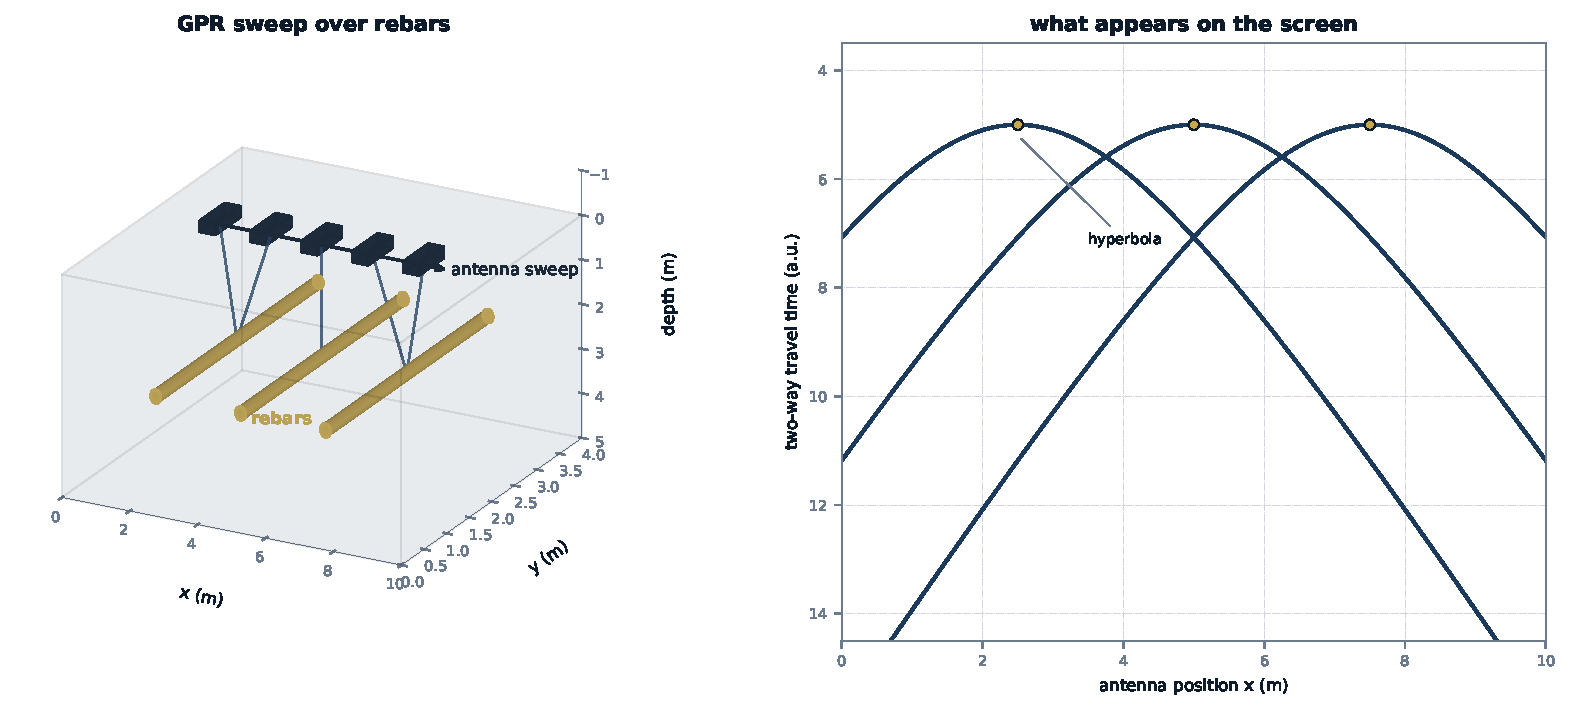
\includegraphics[width=0.98\textwidth,height=0.82\textheight,keepaspectratio]{gpr/hyperbola_viz.pdf}
\end{frame}

\begin{frame}{Wave Speed \& Dielectric Constants}
  \begin{columns}[c]
    \begin{column}{0.5\textwidth}\centering
      
\includegraphics[width=0.95\textwidth]{misc/image5.png}
    \end{column}
    \begin{column}{0.5\textwidth}
      \begin{tikzpicture}[remember picture, overlay]
        \node[anchor=center] at ([xshift=0.25\textwidth, yshift=0.8cm]current page.center) {%
          \color{navymid}$\displaystyle v \;=\; \frac{c}{\sqrt{\varepsilon_r}}$%
        };
      \end{tikzpicture}
      \vspace{3.2cm}

      {\small $c$ = speed of light}\\[0.4em]
      {\small $\varepsilon_r$ = dielectric constant}\\[1.0em]
      {\footnotesize\color{mutedtext}Time-of-flight gives depth; amplitude gives material contrast.}
    \end{column}
  \end{columns}
\end{frame}

% ═════════════════════════════════════════════════════════════════════════════
% READING RADARGRAMS
% ═════════════════════════════════════════════════════════════════════════════
\begin{frame}{A Raw B-Scan Radargram}
  \centering
  
\includegraphics[width=0.78\textwidth]{misc/image10.png}\\[0.3em]
\end{frame}

\begin{frame}{Reading a Radargram}
  \centering
  
\includegraphics[width=0.78\textwidth]{misc/image4.png}
\end{frame}

% ═════════════════════════════════════════════════════════════════════════════
% AI PRIMER
% ═════════════════════════════════════════════════════════════════════════════
\begin{frame}[plain]
  \vspace{2.8cm}\centering
  {\Huge\color{navydark}\textbf{AI Primer}}\\[0.5em]
  {\color{navymid} How a neural network learns to see}
\end{frame}

\begin{frame}{What Is a Neural Network?}
  \centering
  
\includegraphics[width=0.78\textwidth]{misc/image7.png}\\[0.3em]
  {\footnotesize\color{mutedtext}Labeled examples in $\to$ pattern-matching machine $\to$ class labels out}
\end{frame}

\begin{frame}{Convolutional Neural Network}
  \centering
  
\includegraphics[width=0.85\textwidth]{misc/image16.png}\\[0.3em]
  {\footnotesize\color{mutedtext}Convolutions + pooling stack up into learned features}
\end{frame}

% ═════════════════════════════════════════════════════════════════════════════
% DATA COLLECTION
% ═════════════════════════════════════════════════════════════════════════════
\begin{frame}[plain]
  \vspace{2.8cm}\centering
  {\Huge\color{navydark}\textbf{Methodology}}\\[0.5em]
  {\color{navymid} Data, models, and detection}
\end{frame}

\begin{frame}{Two Machines}
  \begin{columns}[c]
    \begin{column}{0.5\textwidth}\centering
\includegraphics[width=0.85\textwidth]{misc/image20.png}\\{\footnotesize GSSI }\end{column}
    \begin{column}{0.5\textwidth}\centering
\includegraphics[width=0.85\textwidth]{misc/image6.png}\\{\footnotesize Leica GP8000}\end{column}
  \end{columns}
\end{frame}

\begin{frame}{Data Collection at the ERB}
  \centering
  
\includegraphics[width=0.58\textwidth]{misc/image8.png}\\[0.3em]
  {\footnotesize\color{mutedtext}Four hallways, 26-ft passes, 2-ft increments, both machines}
\end{frame}

% ═════════════════════════════════════════════════════════════════════════════
% CONCRETENET
% ═════════════════════════════════════════════════════════════════════════════
% \begin{frame}{The ConcreteNet Pipeline}
%   \centering
%   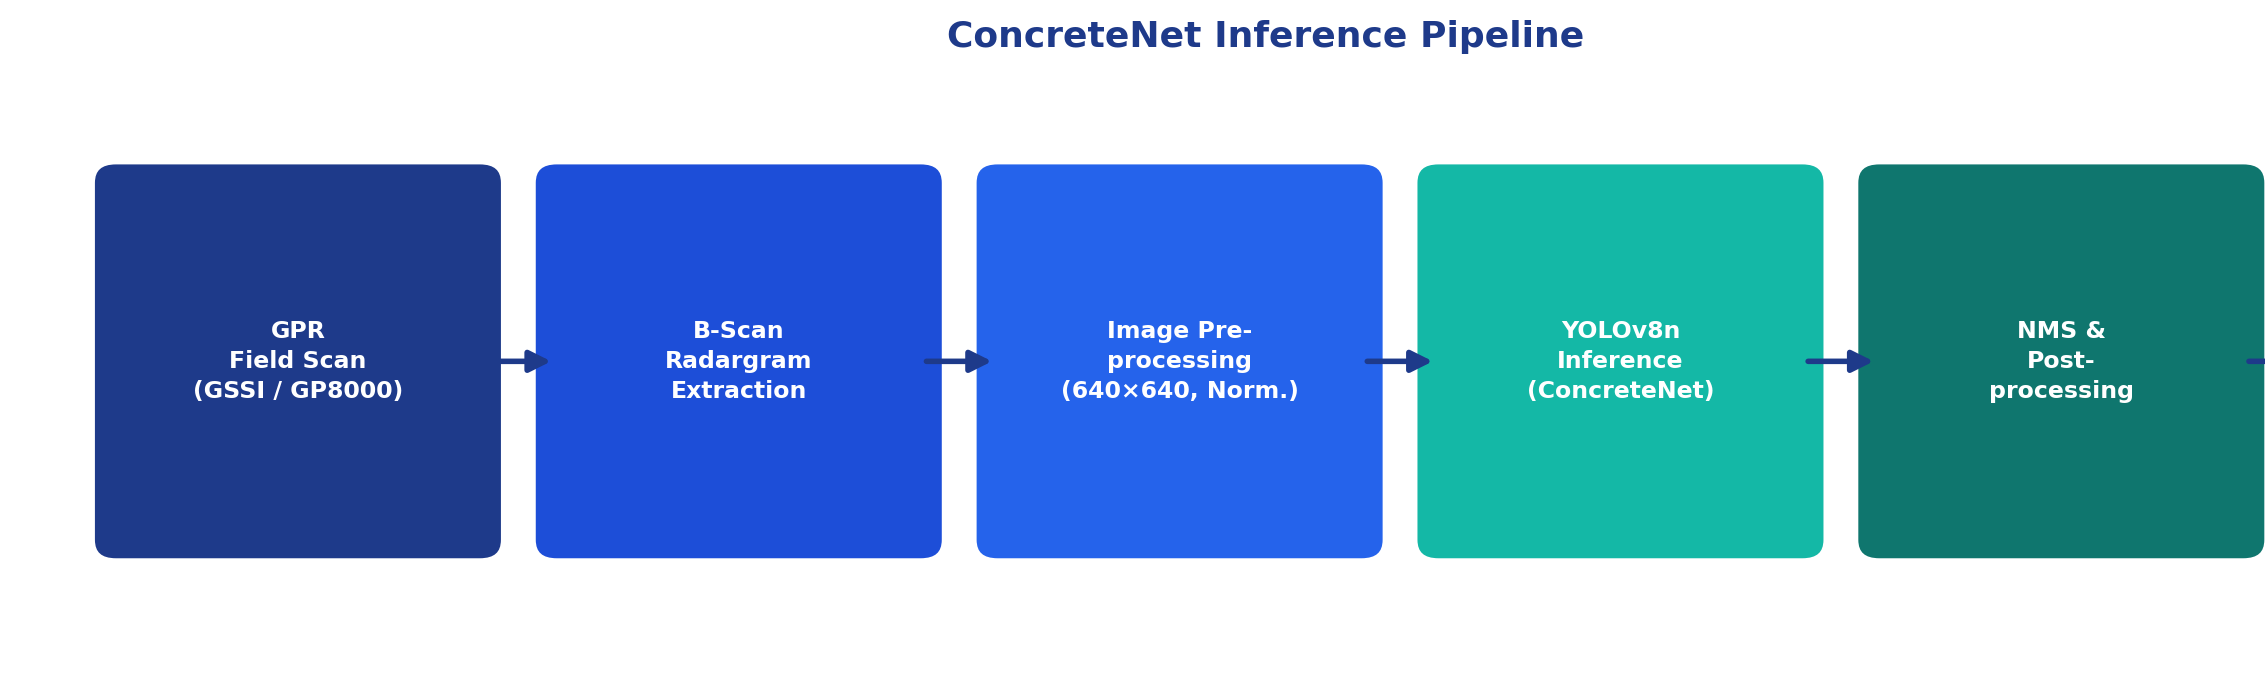
\includegraphics[width=0.9\textwidth]{results/pipeline.png}
% \end{frame}
%
% \begin{frame}{YOLOv8n Architecture}
%   \centering
%   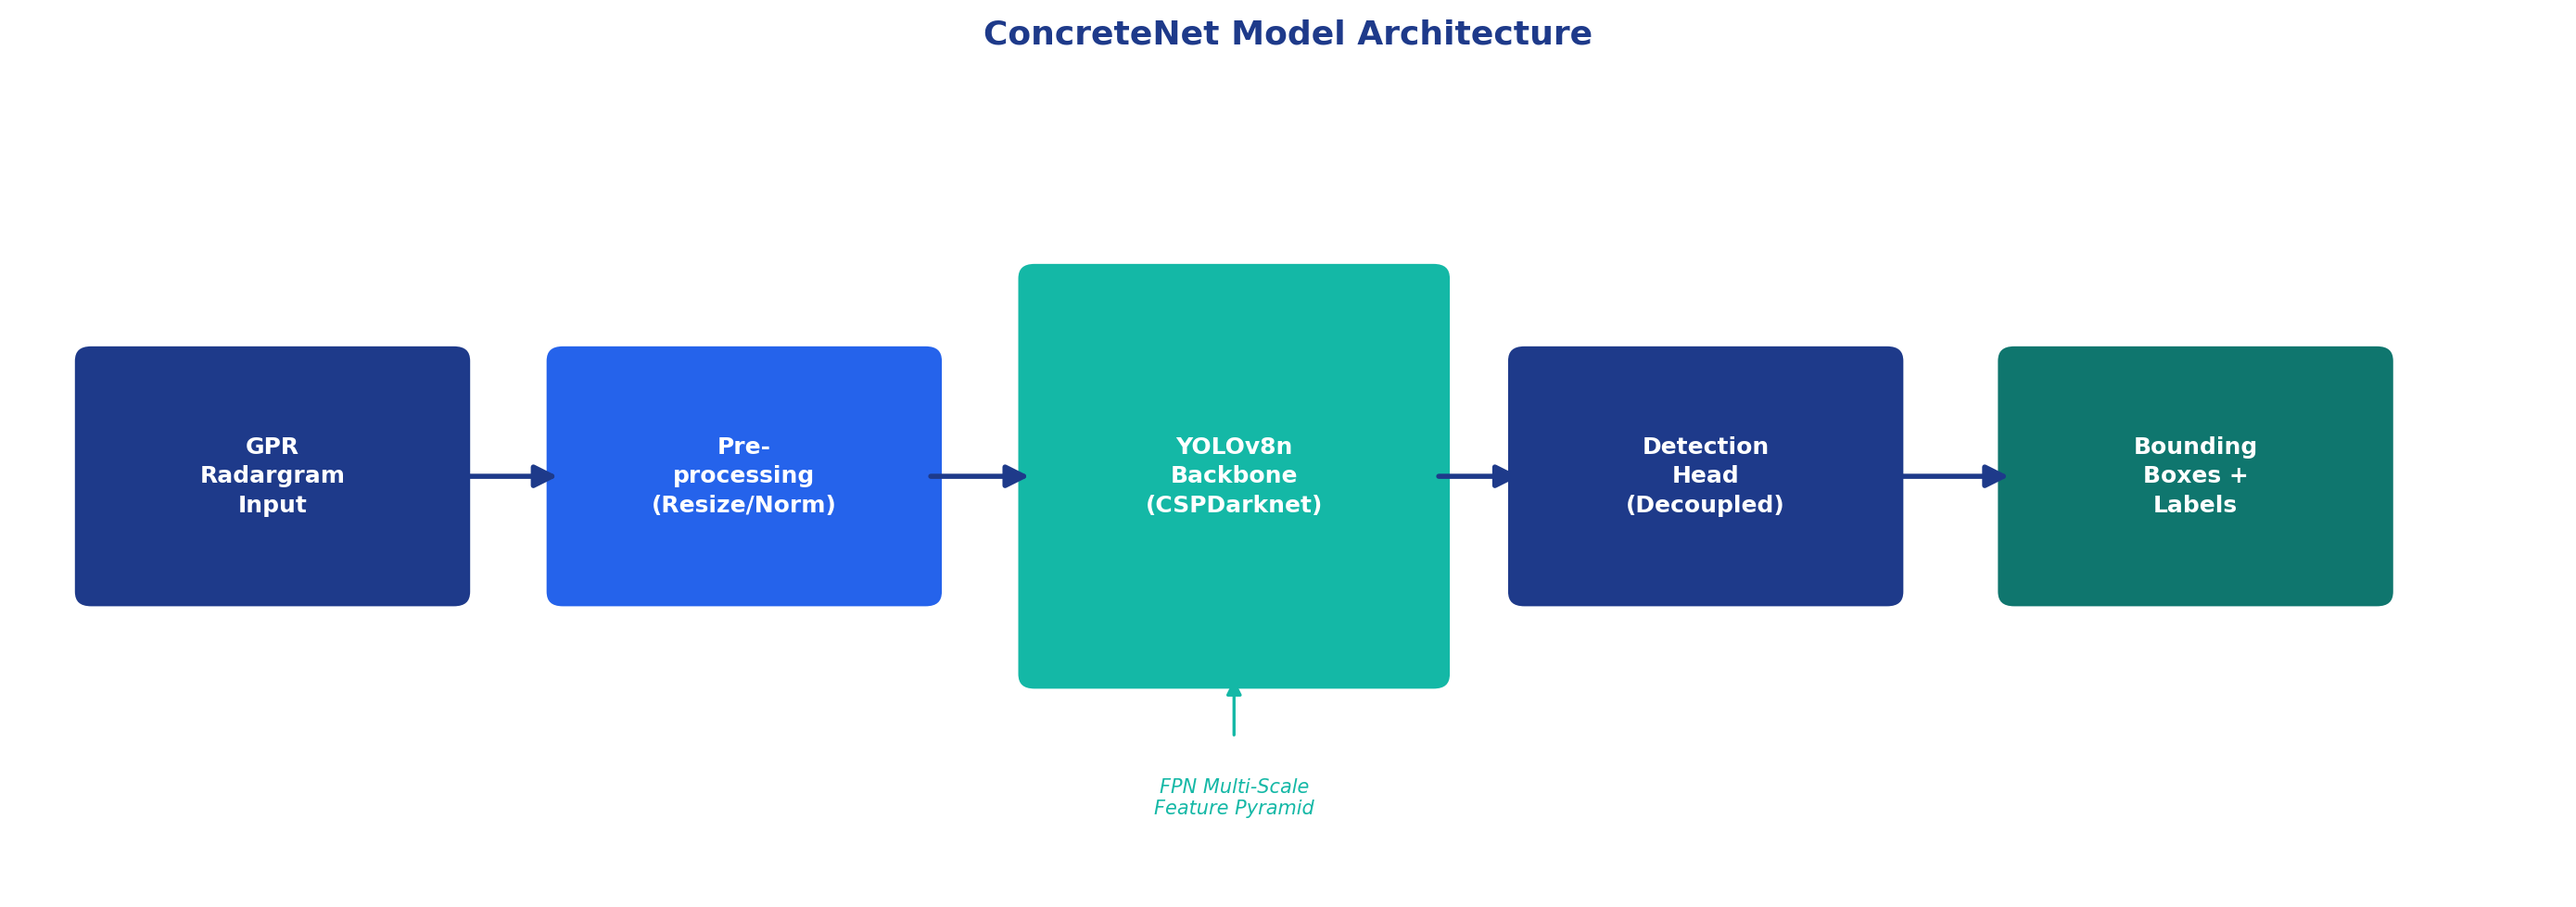
\includegraphics[width=0.78\textwidth]{results/architecture.png}
% \end{frame}

\begin{frame}{Detection Intuition}
  \centering
  
\includegraphics[width=0.78\textwidth]{misc/image17.png}\\[0.3em]
  {\footnotesize\color{mutedtext}Each blue box = one hyperbolic rebar echo}
\end{frame}

% ═════════════════════════════════════════════════════════════════════════════
% RESULTS
% ═════════════════════════════════════════════════════════════════════════════
\begin{frame}{Detections}
  \begin{columns}[c]
    \begin{column}{0.5\textwidth}\centering
      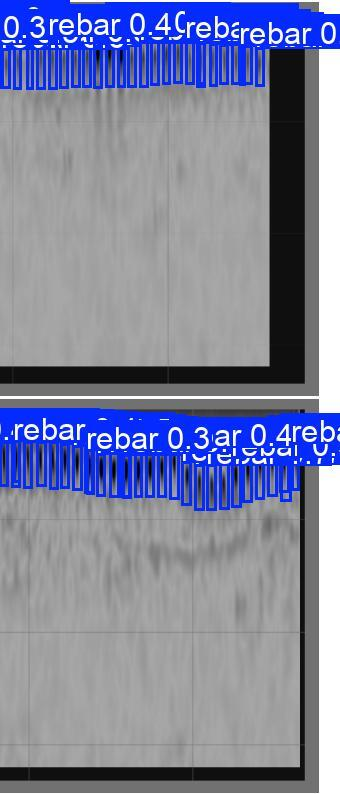
\includegraphics[height=6.8cm,keepaspectratio]{results/gp8000_predictions_crop.jpg}\\[0.3em]
      {\footnotesize\textbf{GP8000}}
    \end{column}
    \begin{column}{0.5\textwidth}\centering
      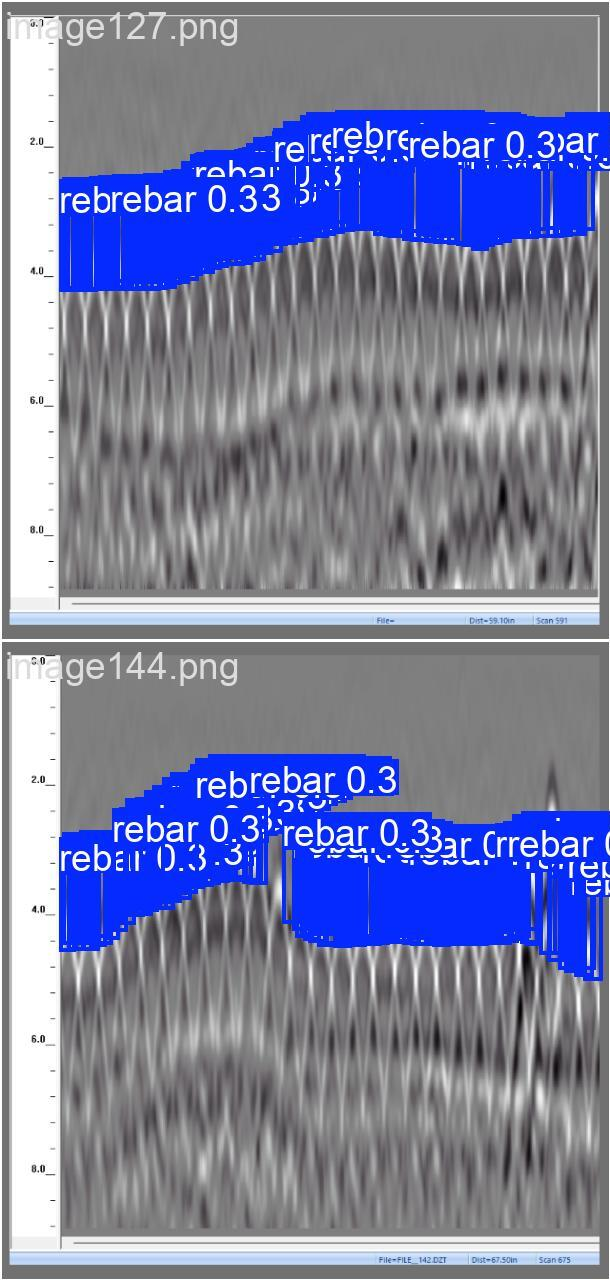
\includegraphics[height=6.8cm,keepaspectratio]{results/gssi_predictions_crop.jpg}\\[0.3em]
      {\footnotesize\textbf{GSSI}}
    \end{column}
  \end{columns}
\end{frame}

% \begin{frame}{Performance --- mAP@0.5}
%   \centering
%   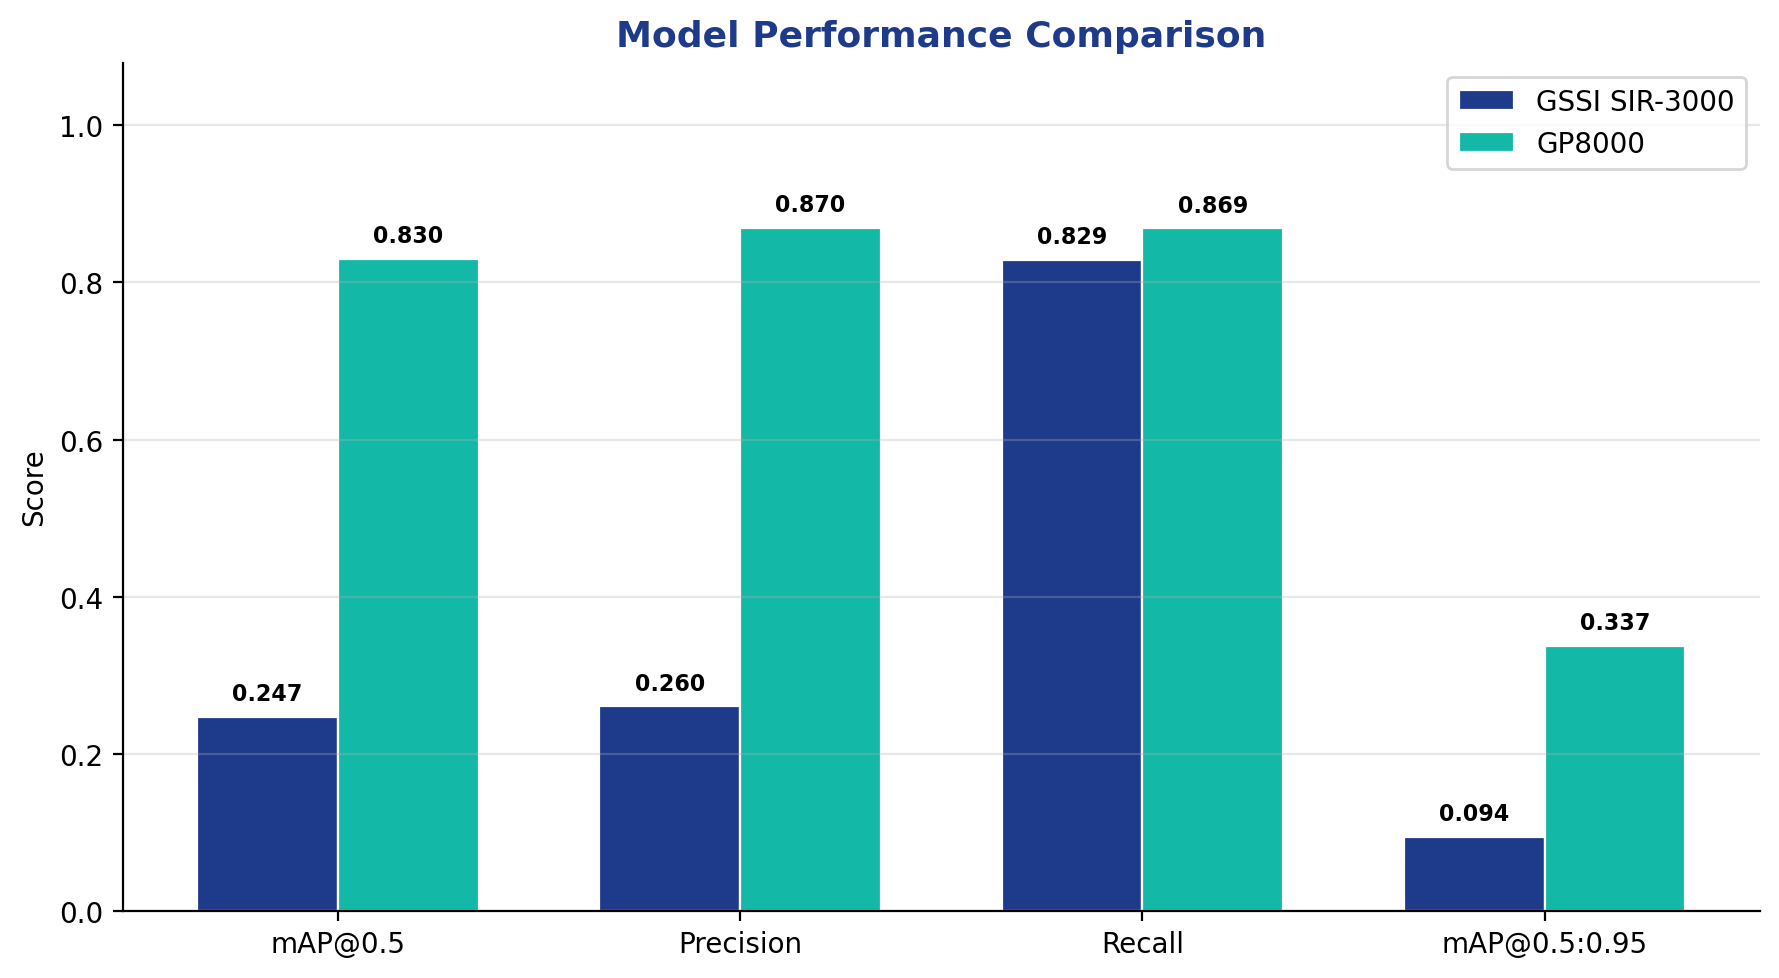
\includegraphics[width=0.72\textwidth]{results/perf_bar.png}
% \end{frame}
%
% \begin{frame}{Training Curves --- GP8000}
%   \centering
%   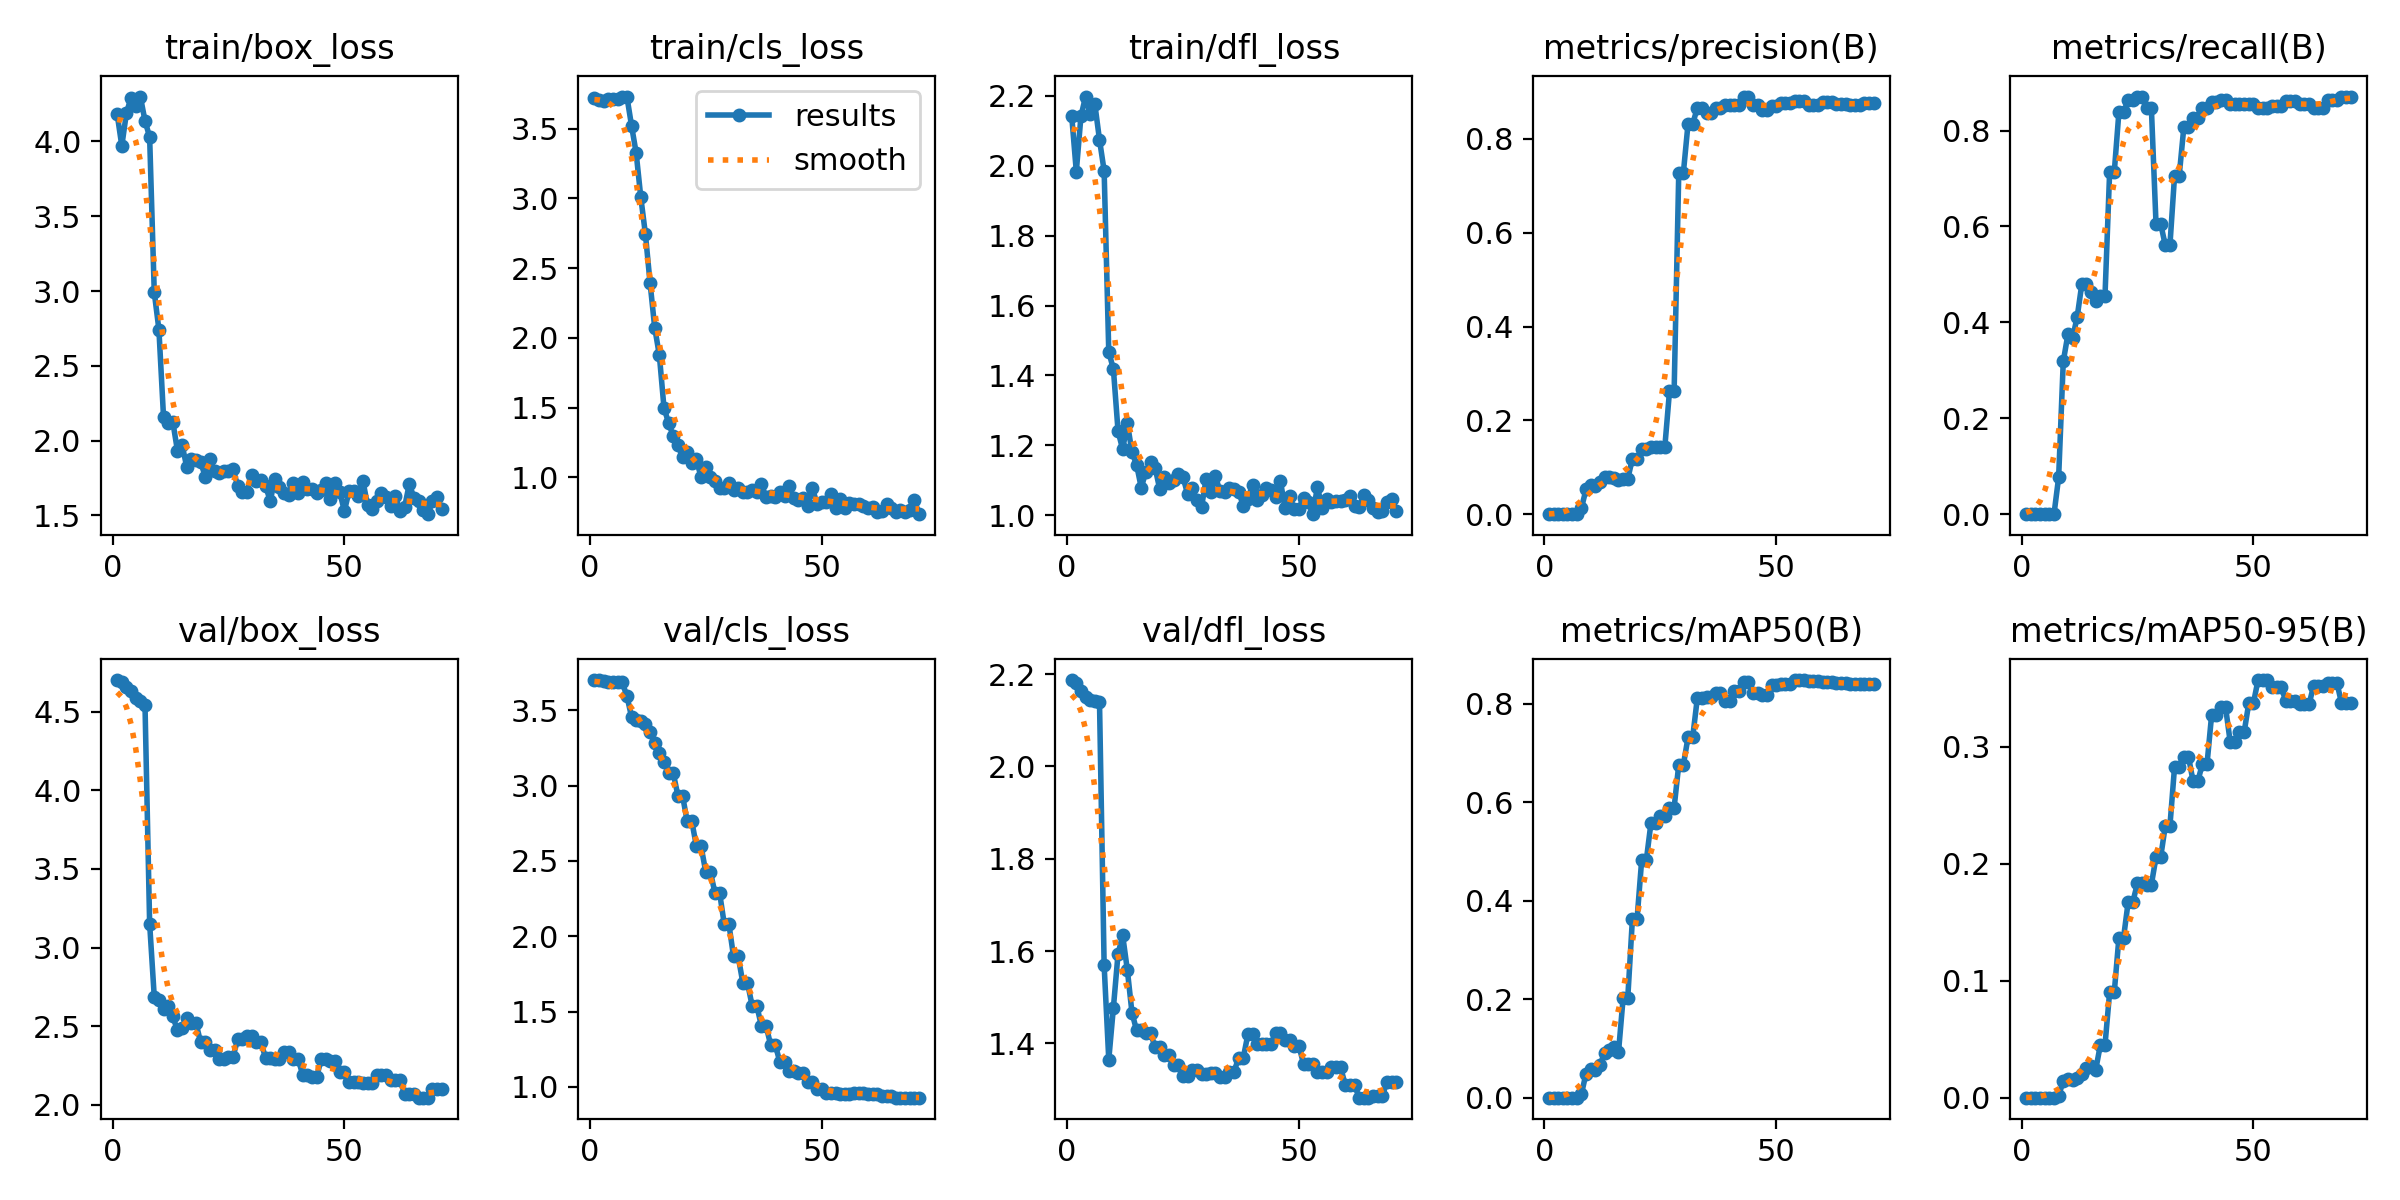
\includegraphics[width=0.95\textwidth]{results/gp8000_results.png}
% \end{frame}

% \begin{frame}{Training Curves --- GSSI}
%   \centering
%   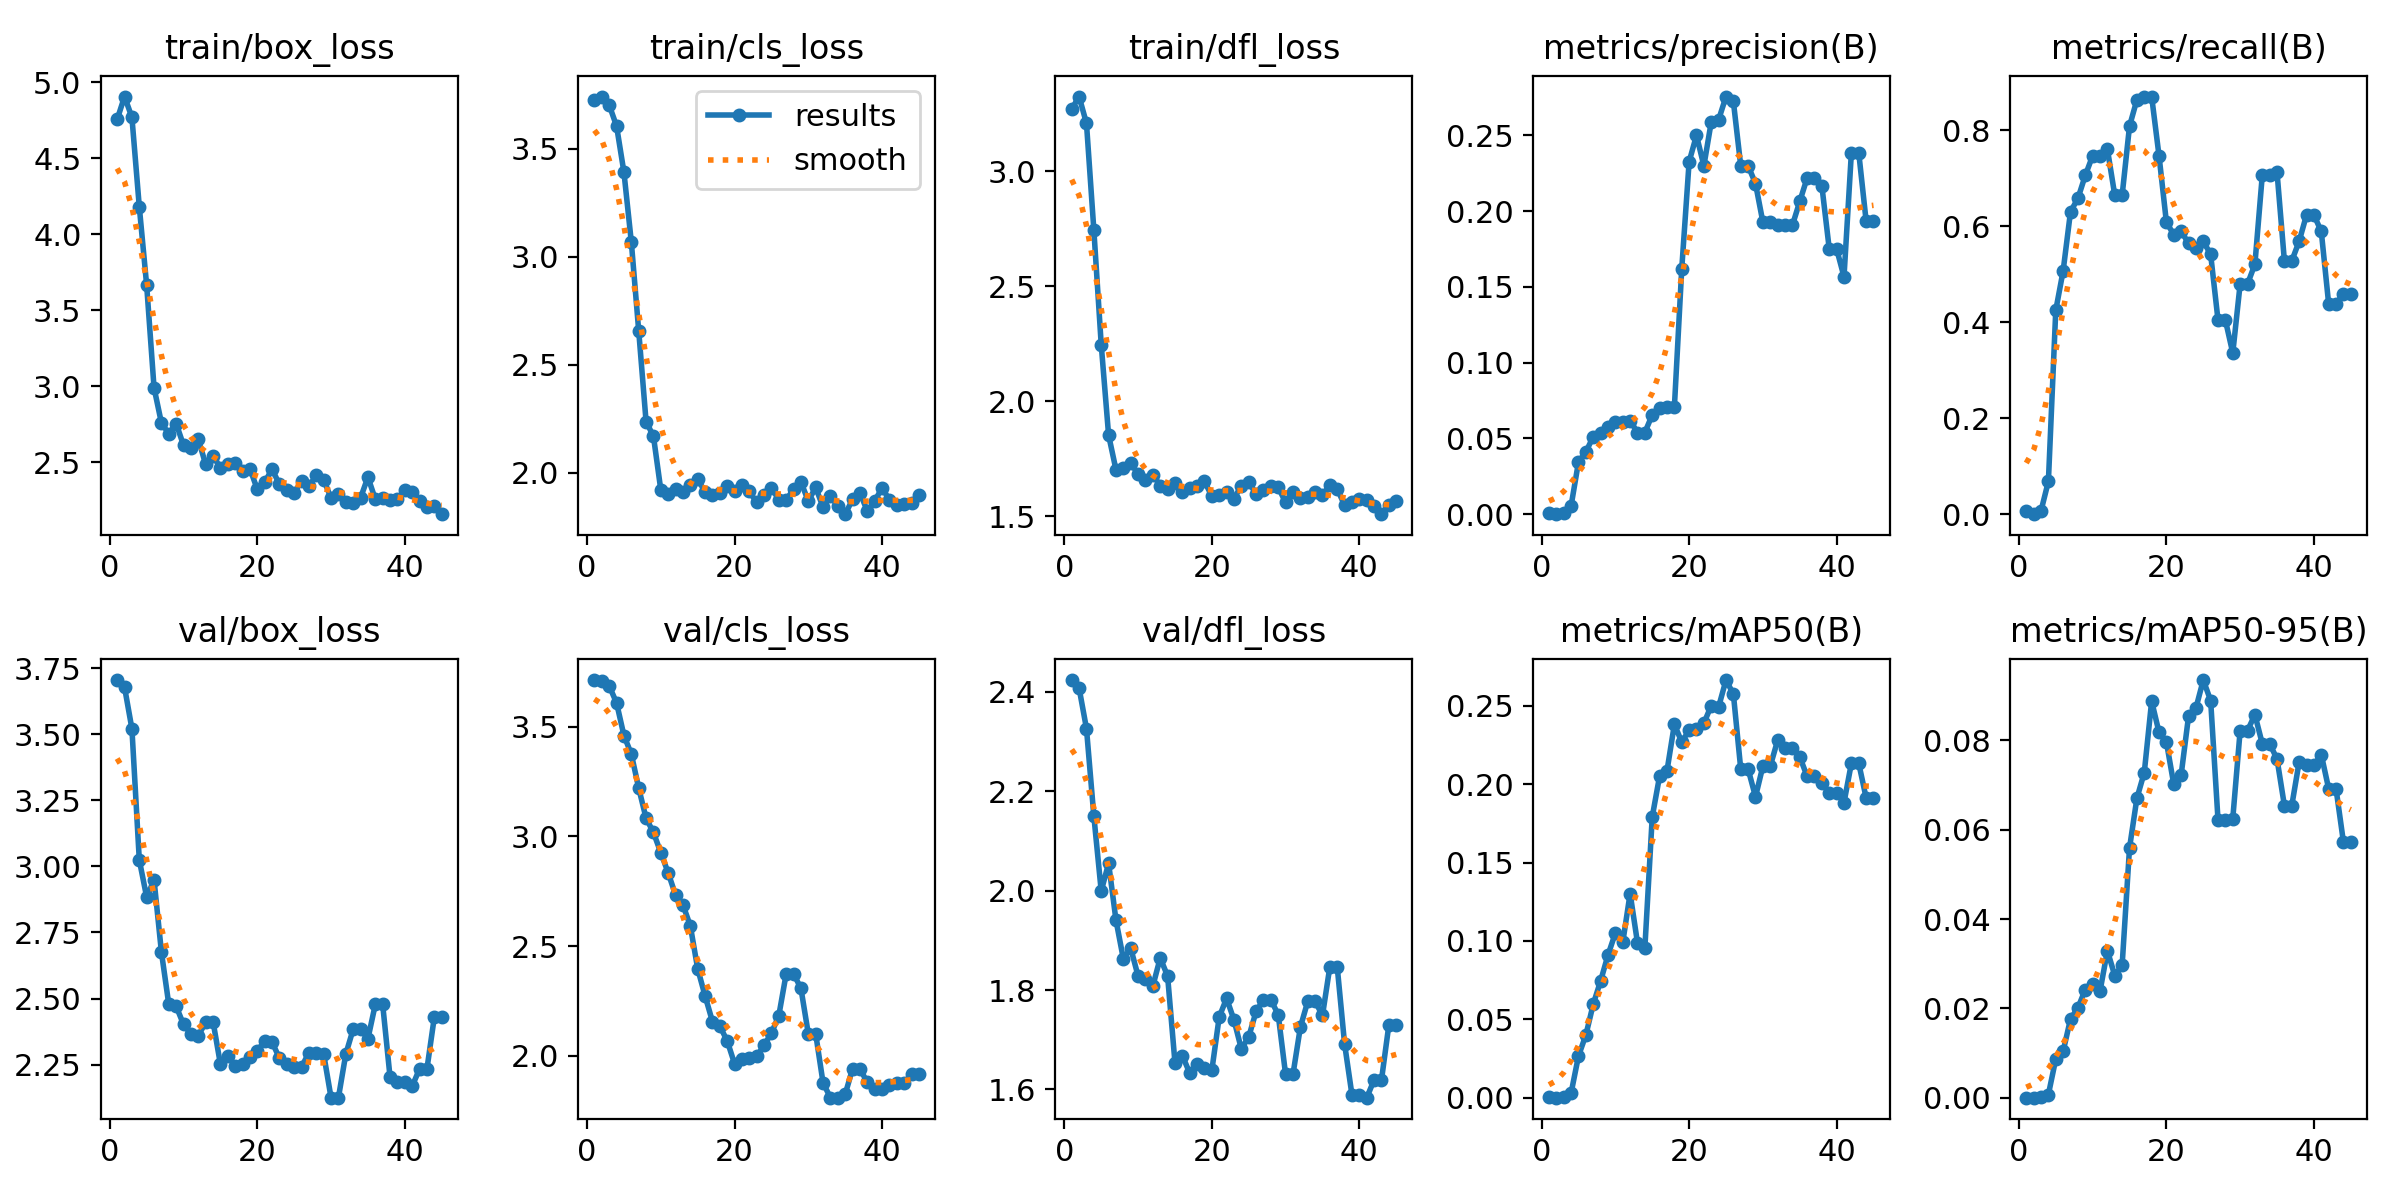
\includegraphics[width=0.95\textwidth]{results/gssi_results.png}
% \end{frame}
%
% \begin{frame}{Precision-Recall --- GP8000}
%   \centering
%   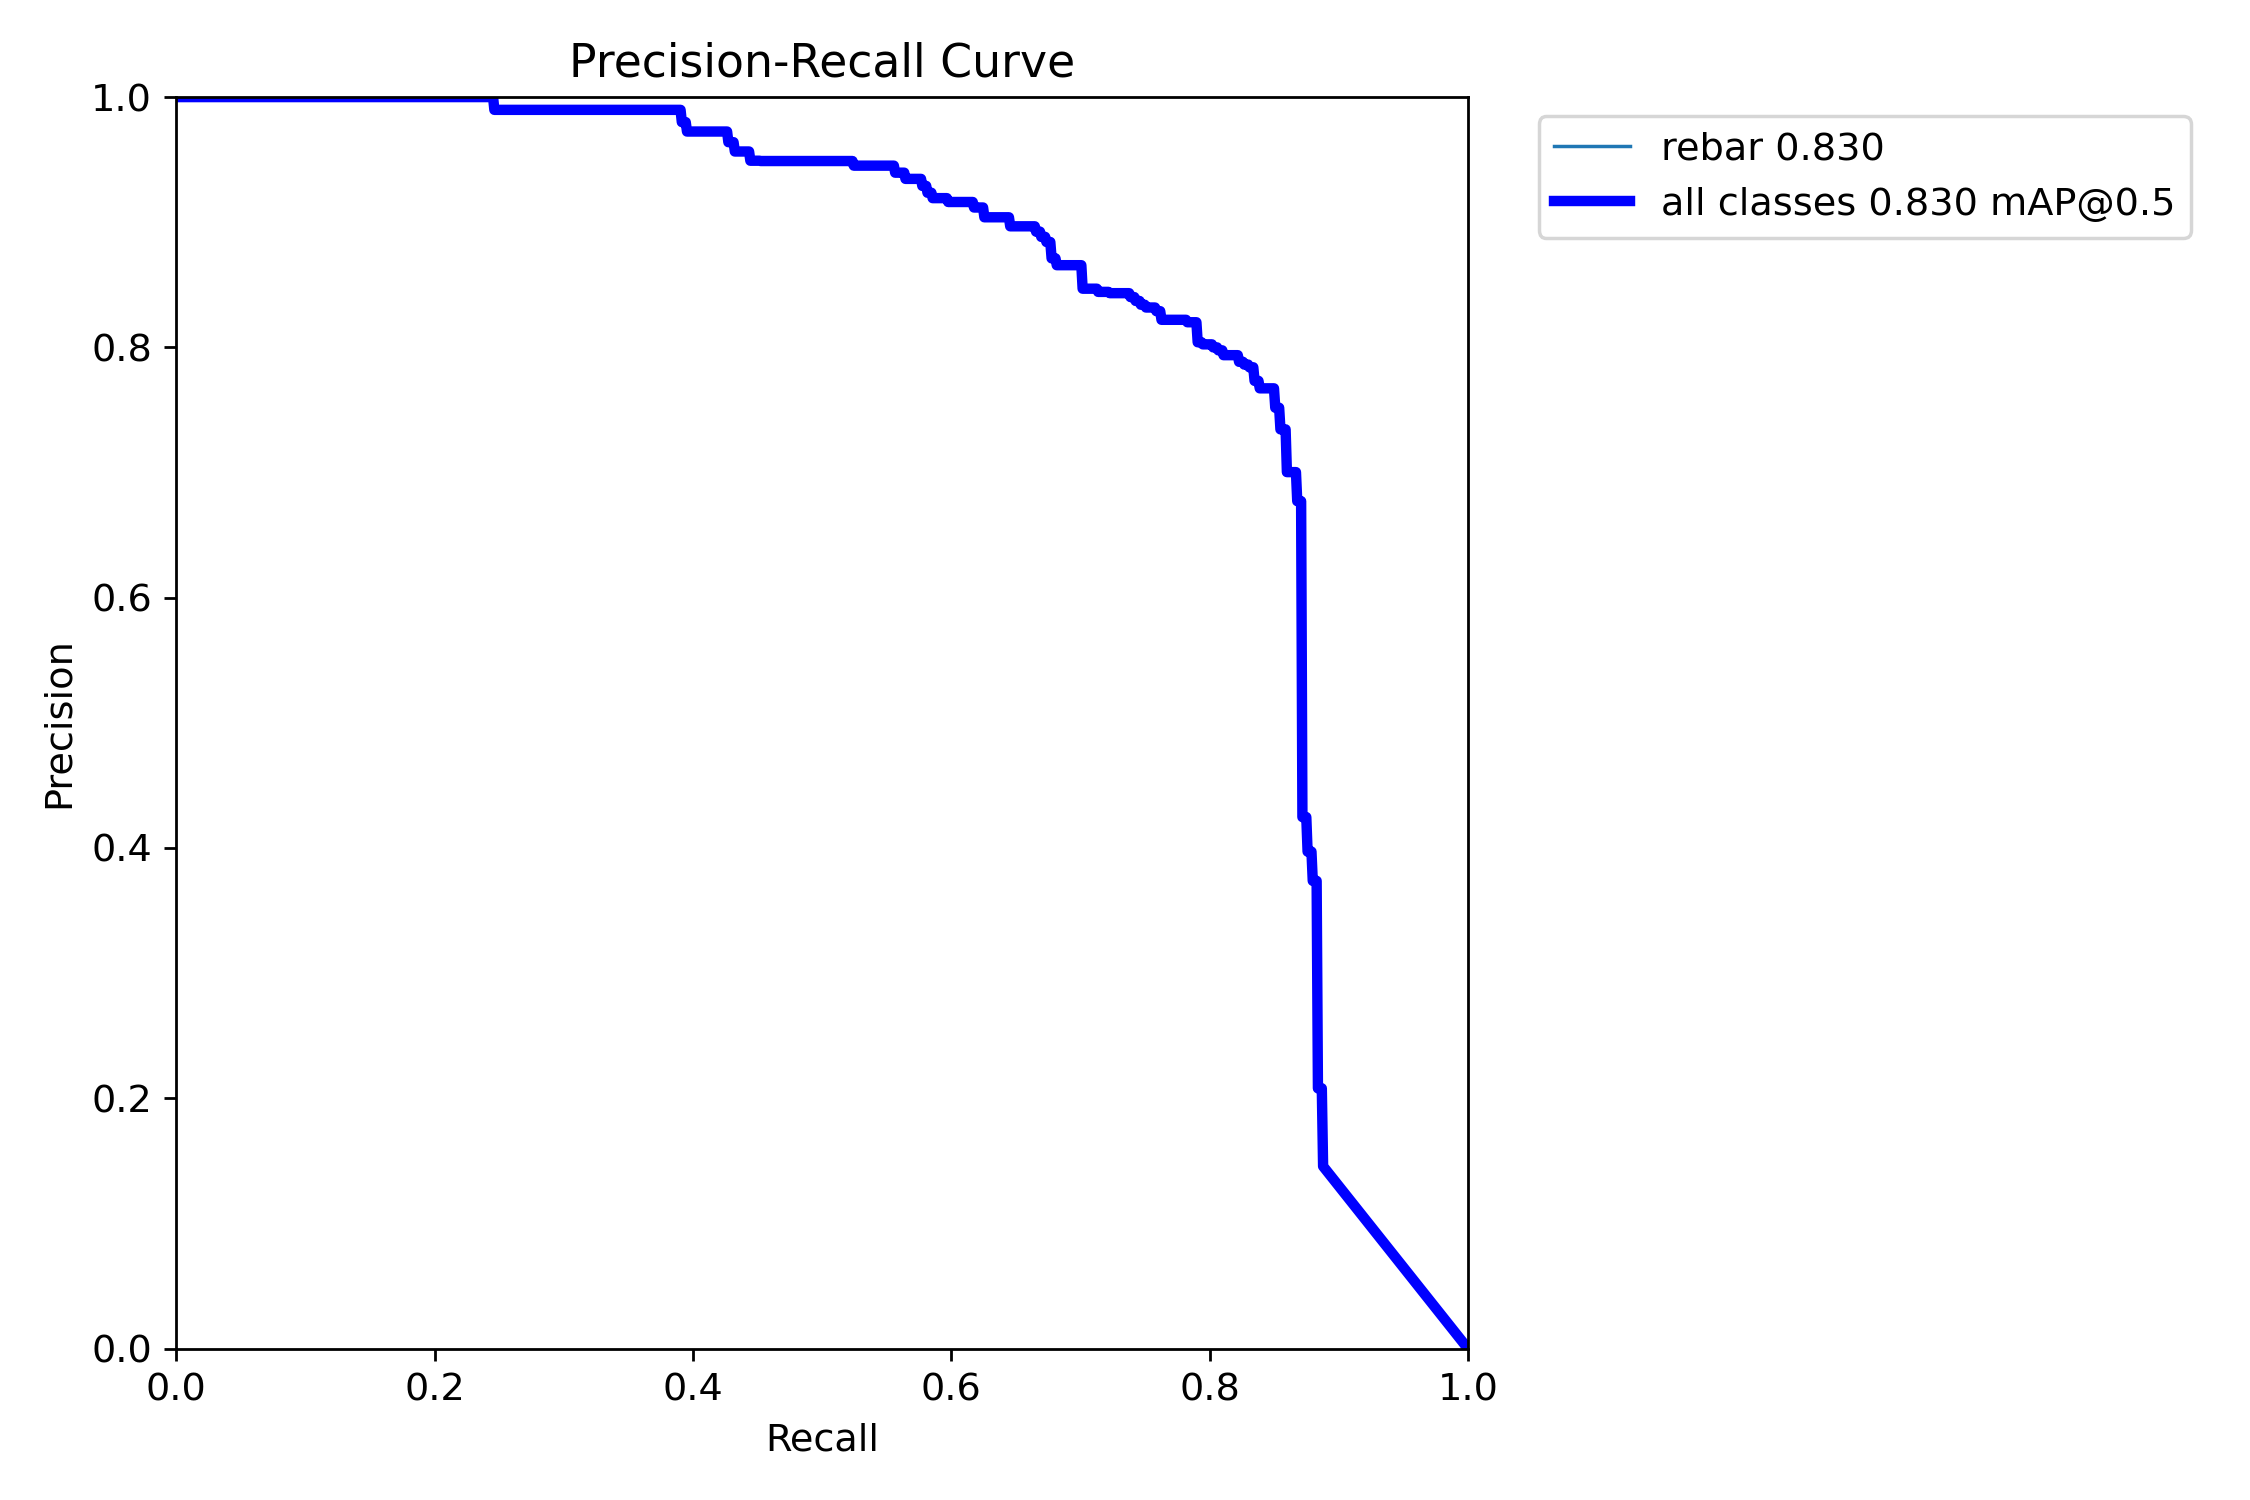
\includegraphics[width=0.72\textwidth]{results/gp8000_pr_curve.png}
% \end{frame}
%
% \begin{frame}{Precision-Recall --- GSSI}
%   \centering
%   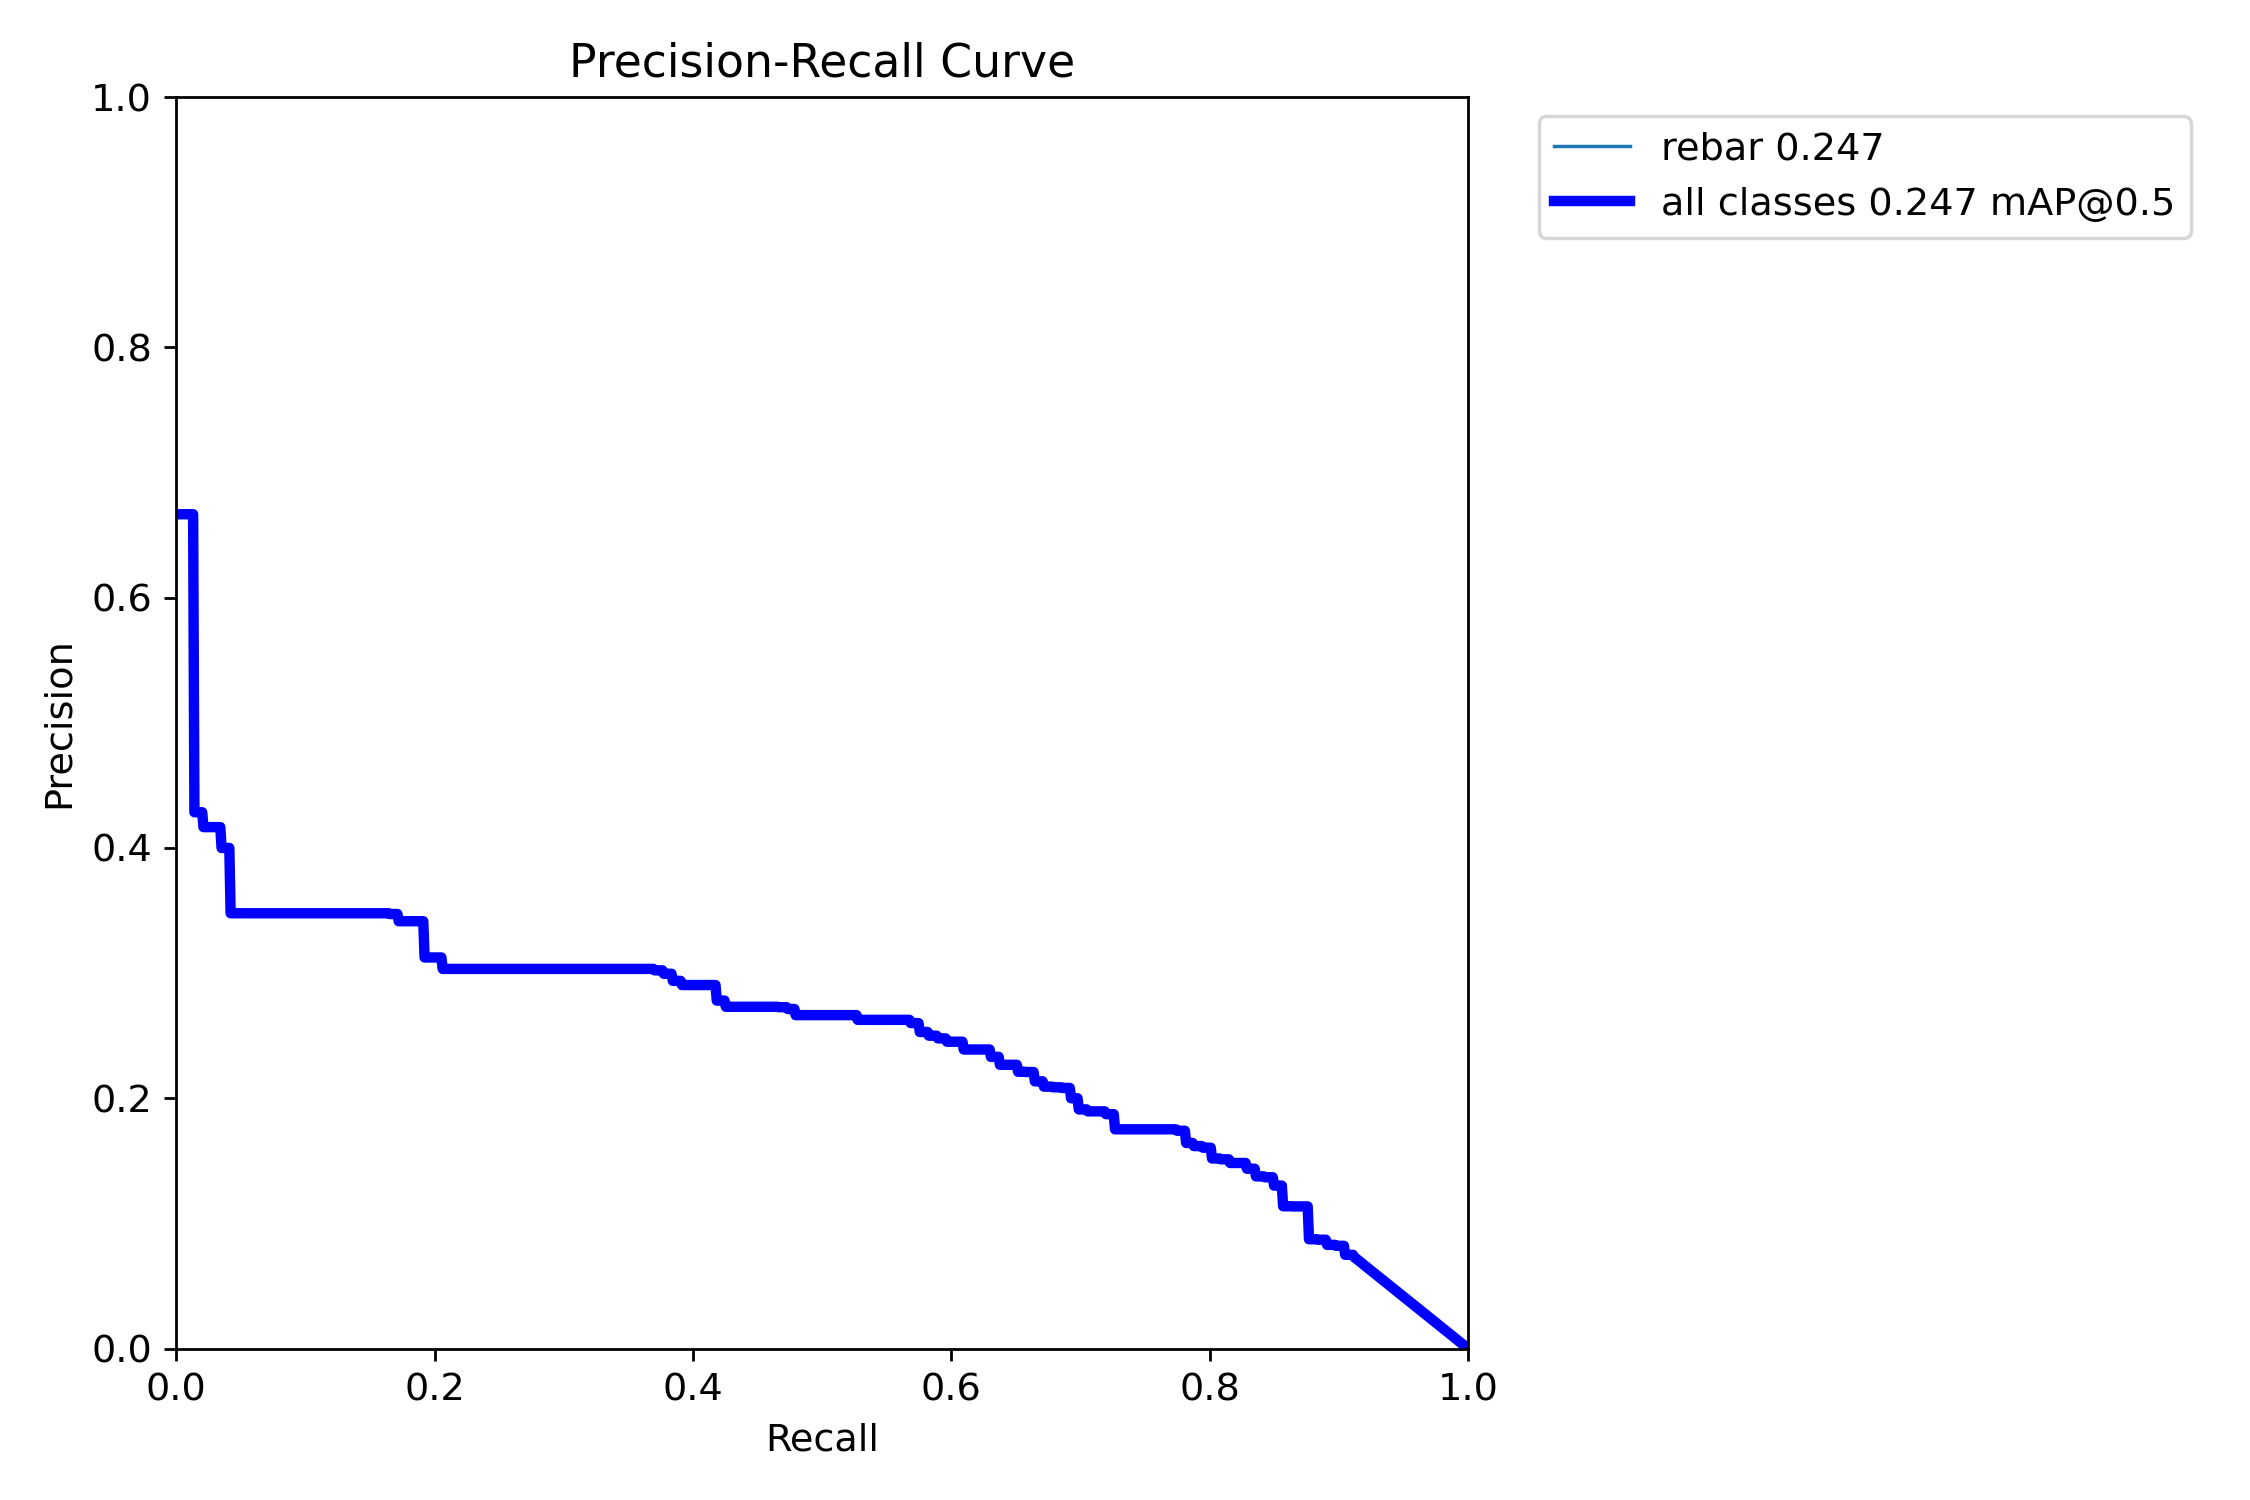
\includegraphics[width=0.72\textwidth]{results/gssi_pr_curve.png}
% \end{frame}

% ═════════════════════════════════════════════════════════════════════════════
% APP DEEP DIVE
% ═════════════════════════════════════════════════════════════════════════════
\begin{frame}[plain]
  \vspace{2.8cm}\centering
  {\Huge\color{navydark}\textbf{The ConcreteNet App}}\\[0.5em]
  {\color{navymid} A desktop tool for field engineers}
\end{frame}

\begin{frame}{Full Window}
  \centering
  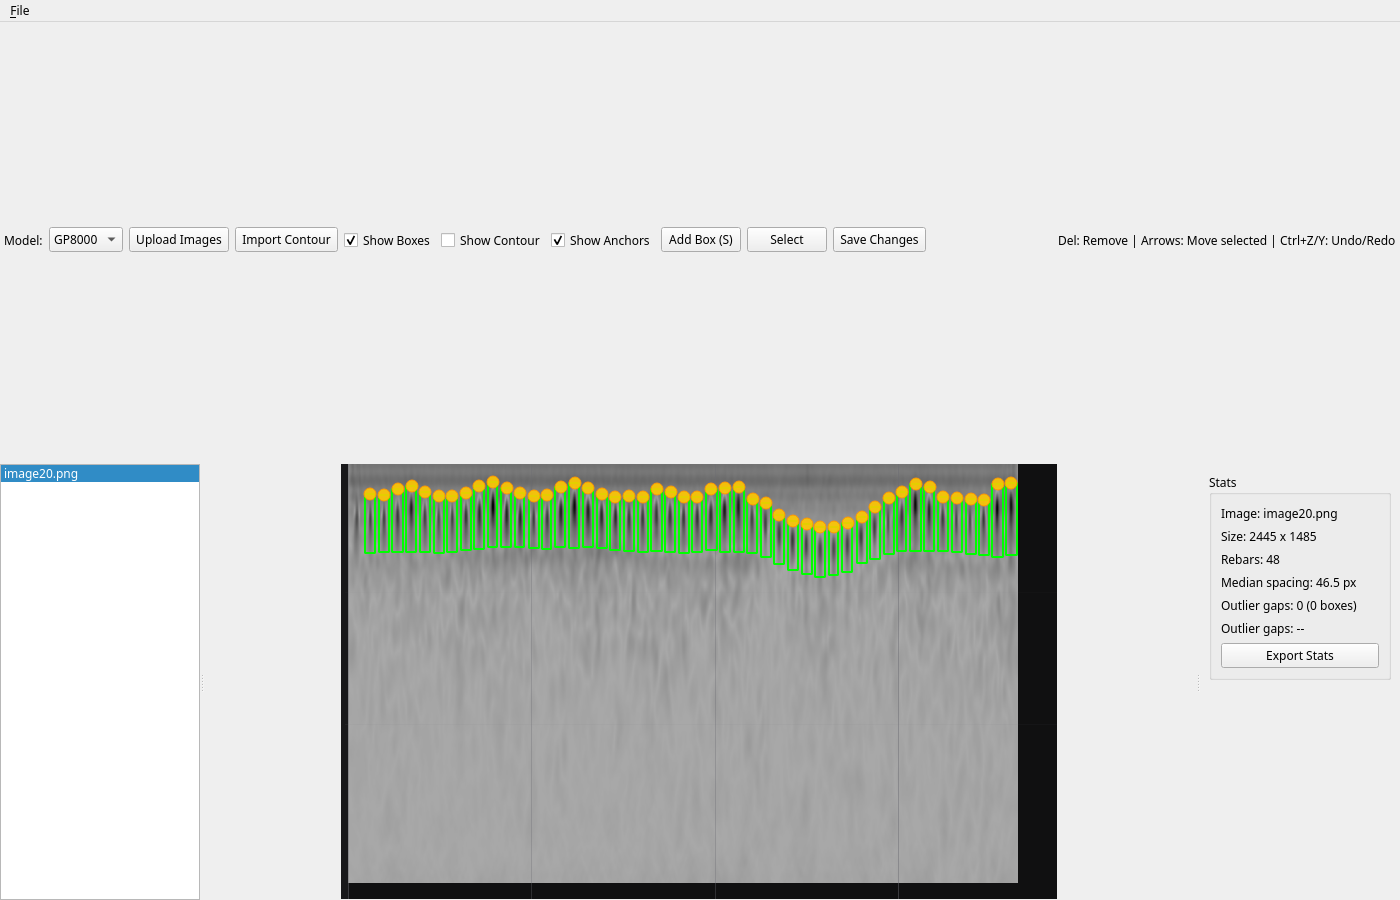
\includegraphics[width=0.98\textwidth]{app/01_full_window.png}
\end{frame}

\begin{frame}{Toolbar}
  \centering
  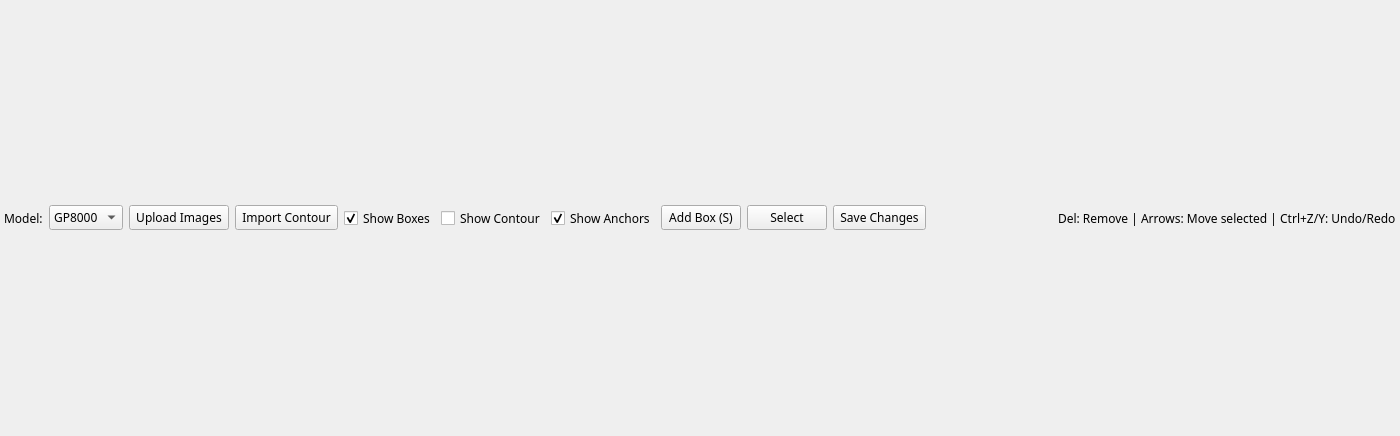
\includegraphics[width=0.98\textwidth,trim=0 180 0 180,clip]{app/02_toolbar.png}\\[0.3em]
  {\footnotesize\color{mutedtext}Model selector \textbullet\ Upload \textbullet\ Import Contour \textbullet\ visibility toggles \textbullet\ Add/Select modes \textbullet\ Save}
\end{frame}

\begin{frame}{Stats and Image List for Projects}
  \begin{columns}[c]
    \begin{column}{0.35\textwidth}\centering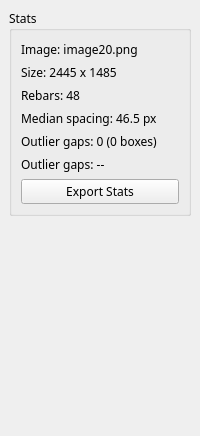
\includegraphics[width=0.95\textwidth]{app/04_stats_panel.png}\end{column}
    \begin{column}{0.6\textwidth}\centering
\includegraphics[width=0.98\textwidth]{app/16_image_list_multi.png}\\[0.3em]{\footnotesize\color{mutedtext}Batch multiple B-scans into one project}\end{column}
  \end{columns}
\end{frame}

\begin{frame}{Canvas --- Auto-Detected Rebars}
  \centering
  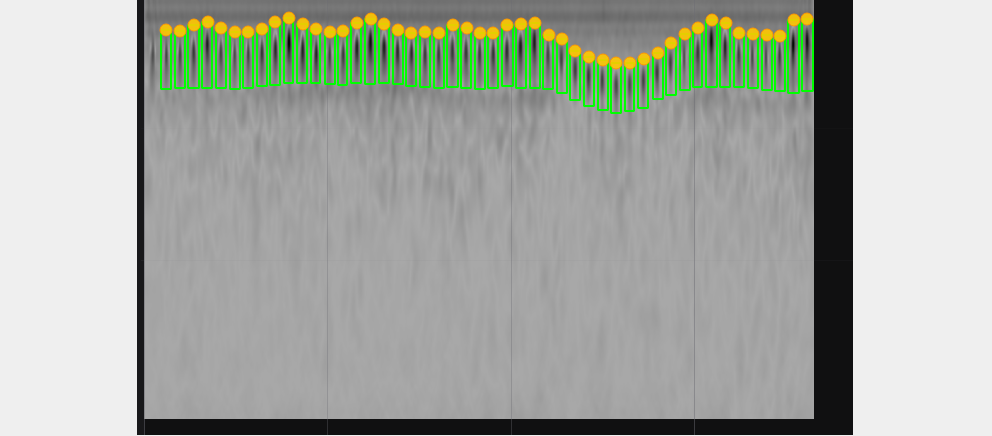
\includegraphics[width=0.95\textwidth]{app/05_canvas_detections.png}\\[0.3em]
  {\footnotesize\color{mutedtext}Green boxes + gold anchor points, one per hyperbolic echo}
\end{frame}

% \begin{frame}{Add Box Mode}
%   \centering
%   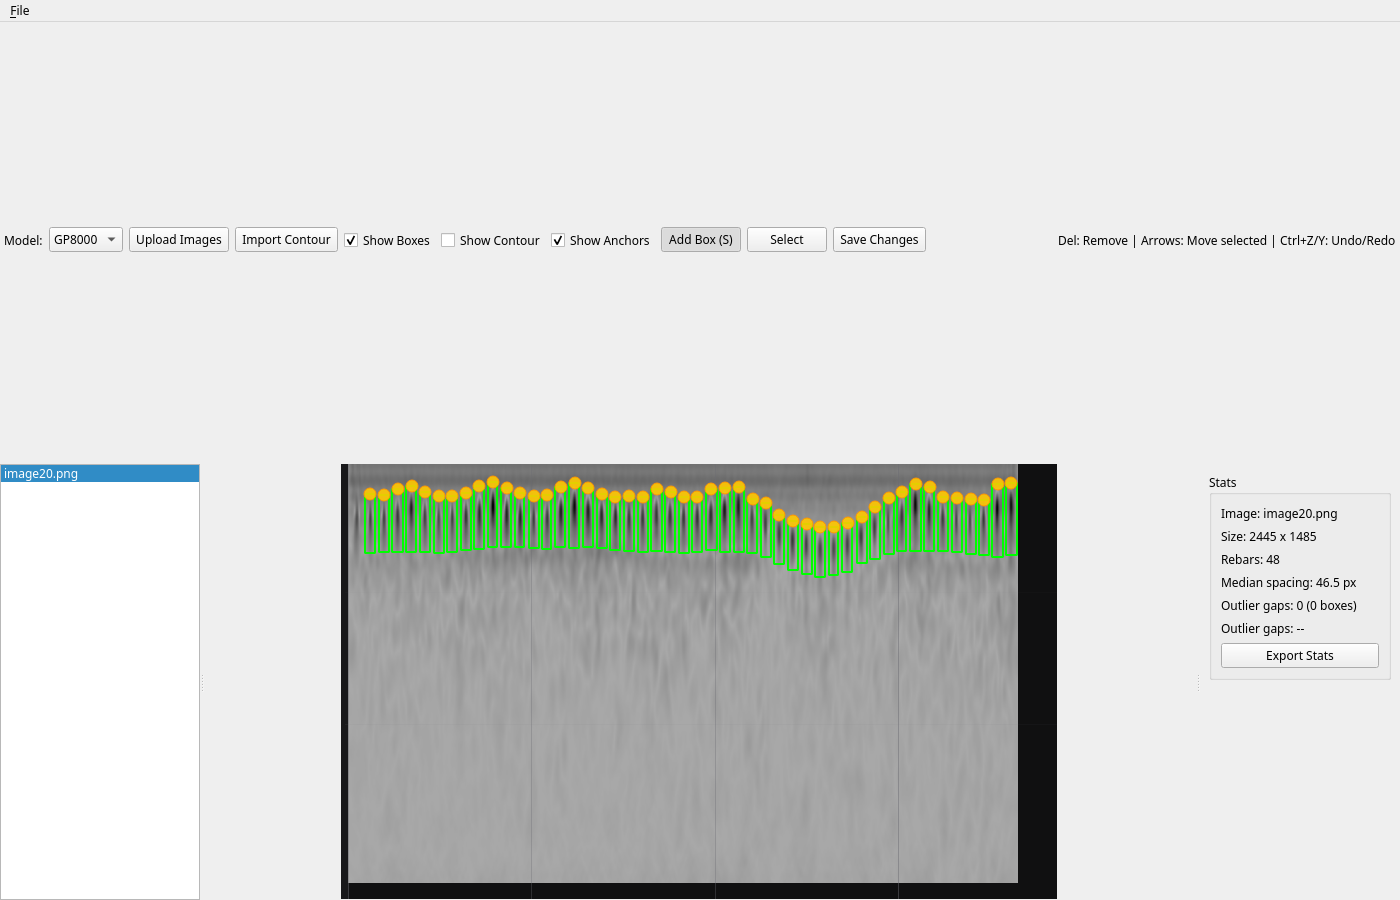
\includegraphics[width=0.95\textwidth]{app/06_add_box_mode.png}\\[0.3em]
%   {\footnotesize\color{mutedtext}\textbf{S} toggles Add mode --- two clicks to place a new rebar box}
% \end{frame}
%
% \begin{frame}{Select Mode --- Multi-Select}
%   \centering
%   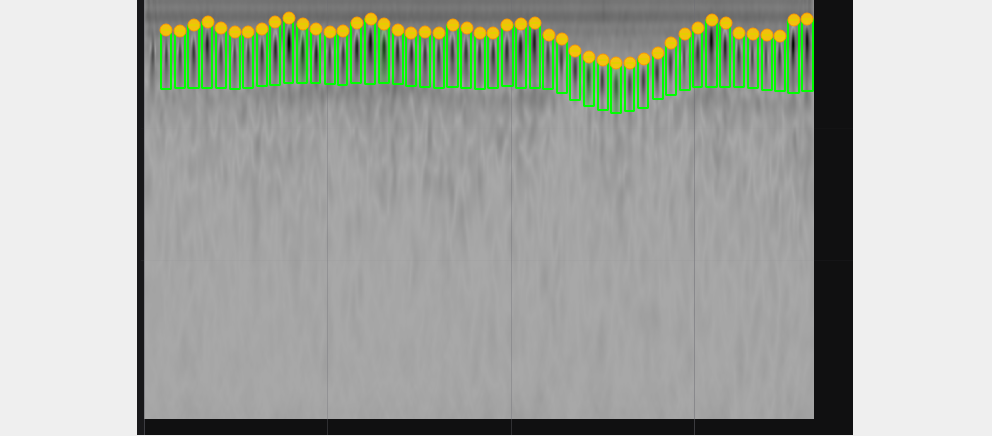
\includegraphics[width=0.95\textwidth]{app/09_canvas_selected.png}\\[0.3em]
%   {\footnotesize\color{mutedtext}Drag-rectangle across multiple rebars; arrow keys move, Del removes}
% \end{frame}

% \begin{frame}{Anchors Only}
%   \centering
%   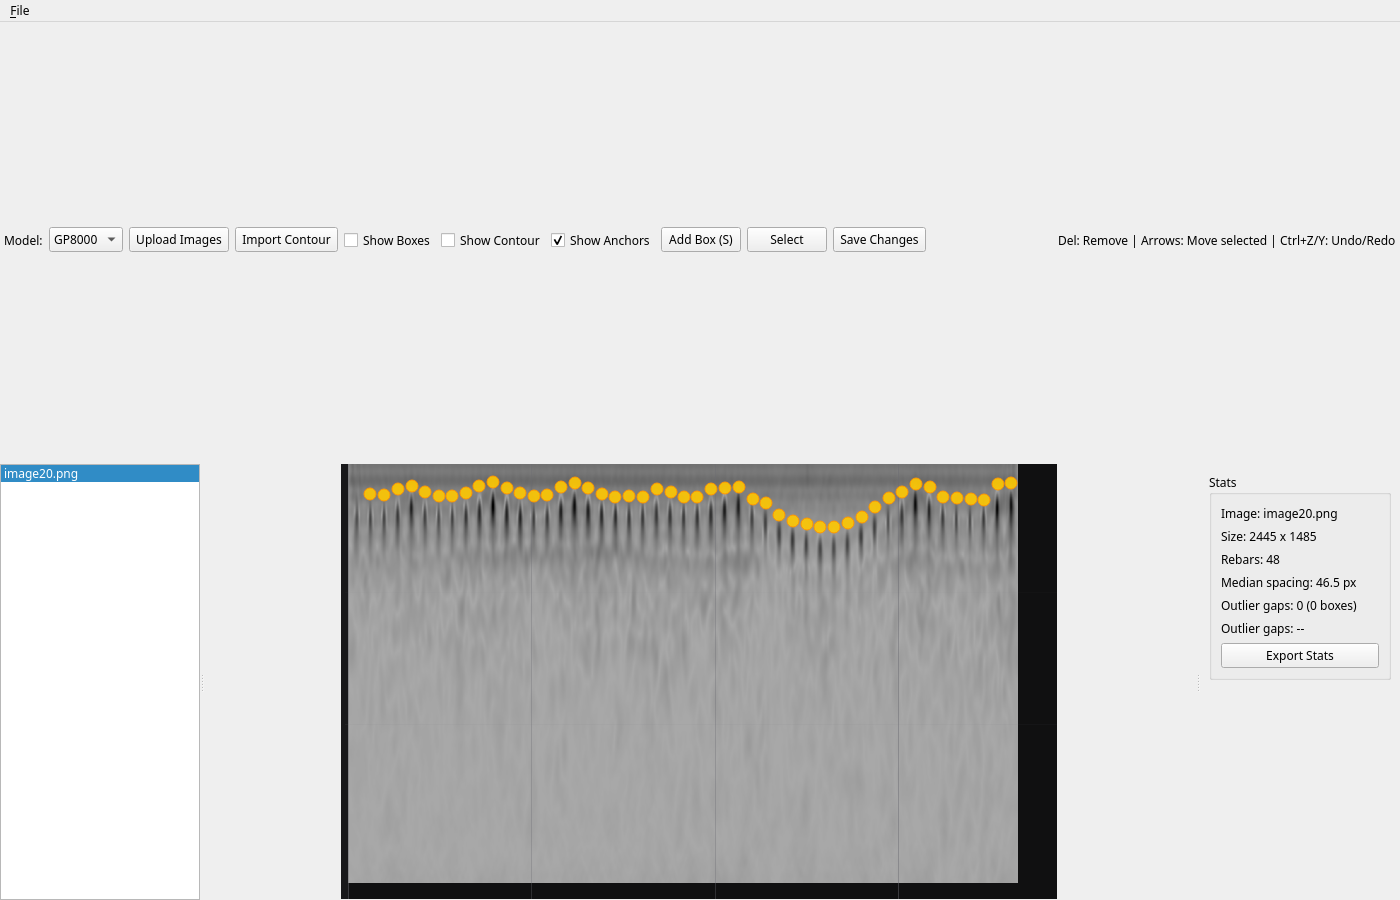
\includegraphics[width=0.95\textwidth]{app/12_anchors_only.png}\\[0.3em]
%   {\footnotesize\color{mutedtext}Hide boxes to focus on the rebar-top anchor track}
% \end{frame}

% \begin{frame}{Rebar-Depth Contour}
%   \centering
%   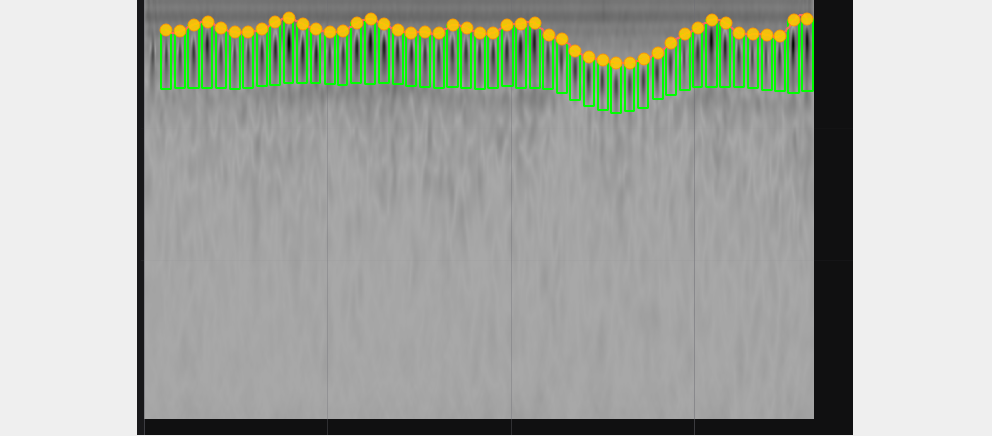
\includegraphics[width=0.95\textwidth]{app/11_canvas_contour.png}\\[0.3em]
%   {\footnotesize\color{mutedtext}Interpolated contour from anchor points}
% \end{frame}

% \begin{frame}{Contour Overlay --- Whole Window}
%   \centering
%   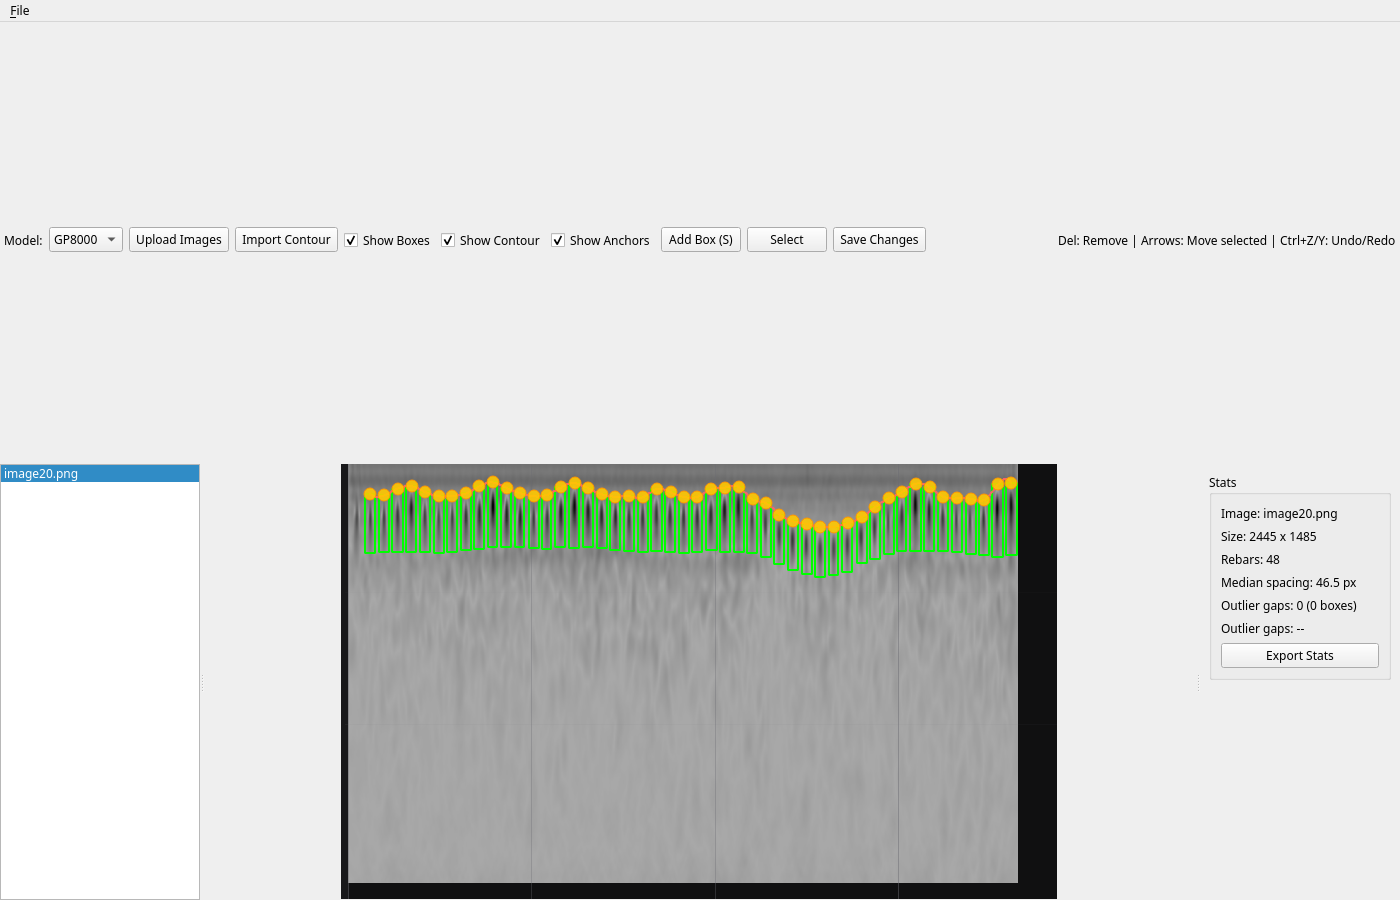
\includegraphics[width=0.95\textwidth]{app/10_contour_overlay.png}
% \end{frame}

\begin{frame}{Contour Overlays Across Years}
  \centering
  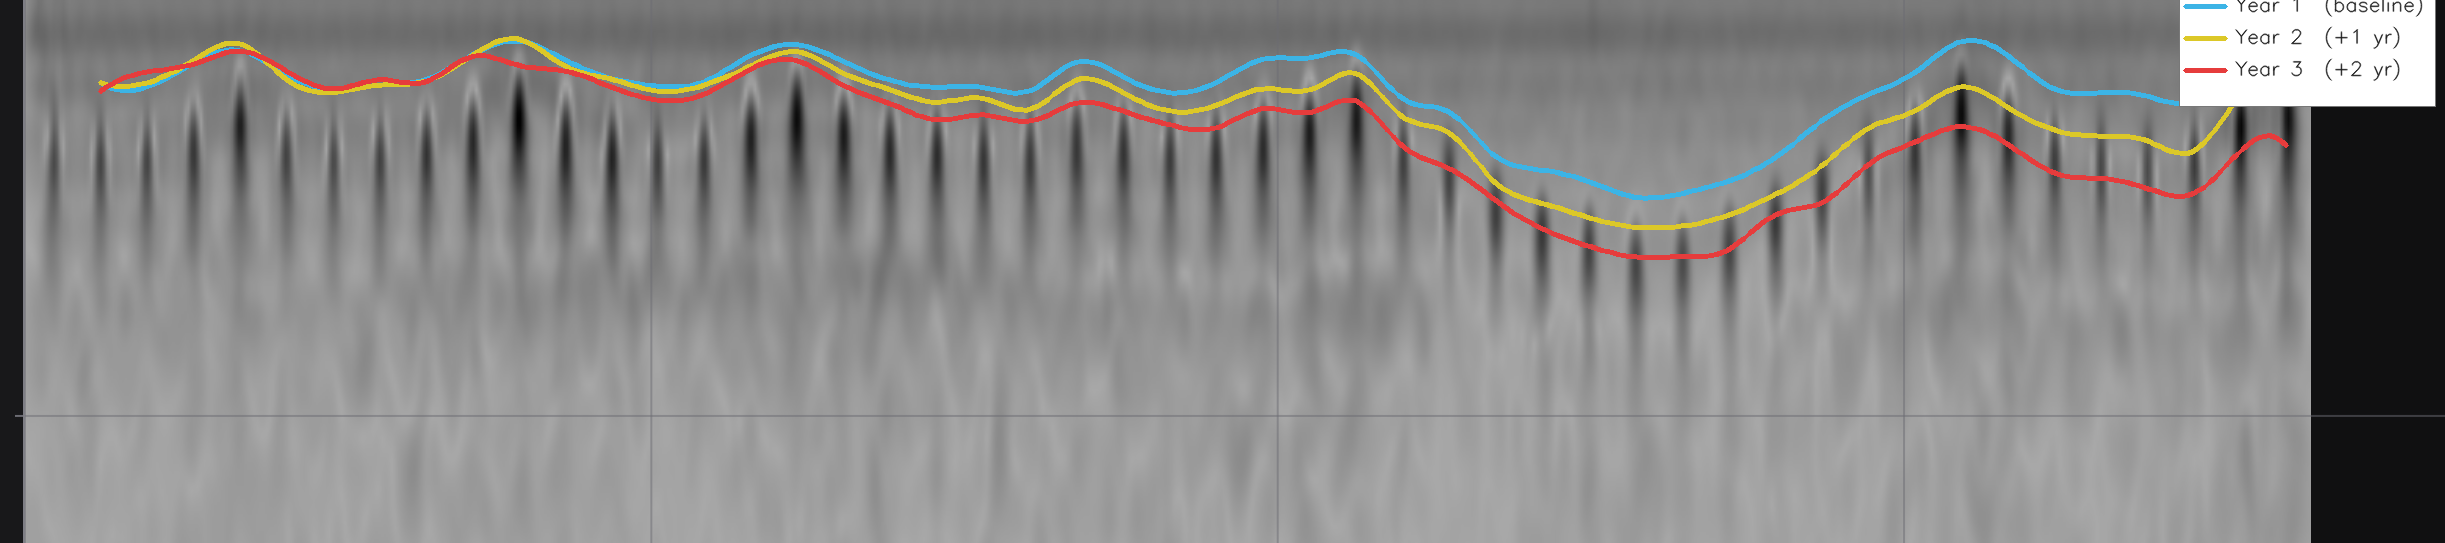
\includegraphics[width=0.98\textwidth]{app/contour_years.png}\\[0.4em]
  {\footnotesize\color{mutedtext}Re-scan the same deck yearly; overlay saved contour JSONs on any image in the project to see rebar-layer drift over time}
\end{frame}

\begin{frame}{Switching Models --- GSSI}
  \centering
  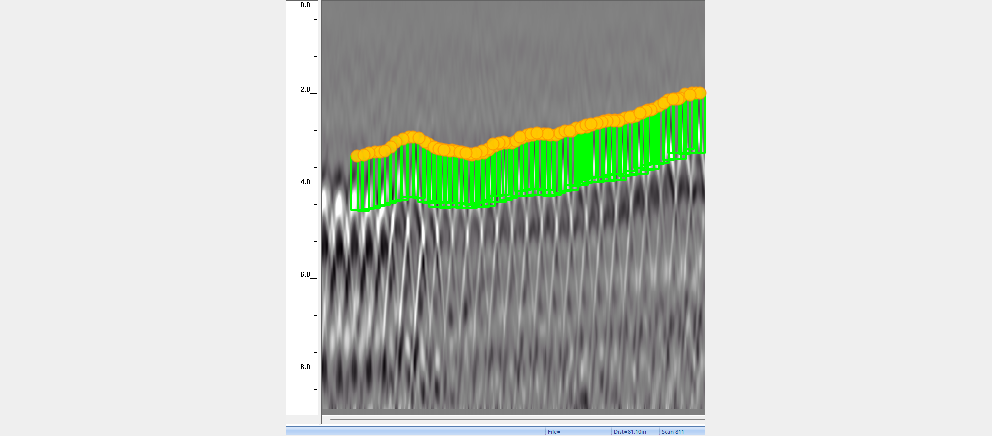
\includegraphics[width=0.95\textwidth]{app/14_gssi_canvas.png}\\[0.3em]
  {\footnotesize\color{mutedtext}Same app, GSSI model loaded, 99 rebars on a GSSI B-scan}
\end{frame}

% \begin{frame}{GSSI --- Full Window}
%   \centering
%   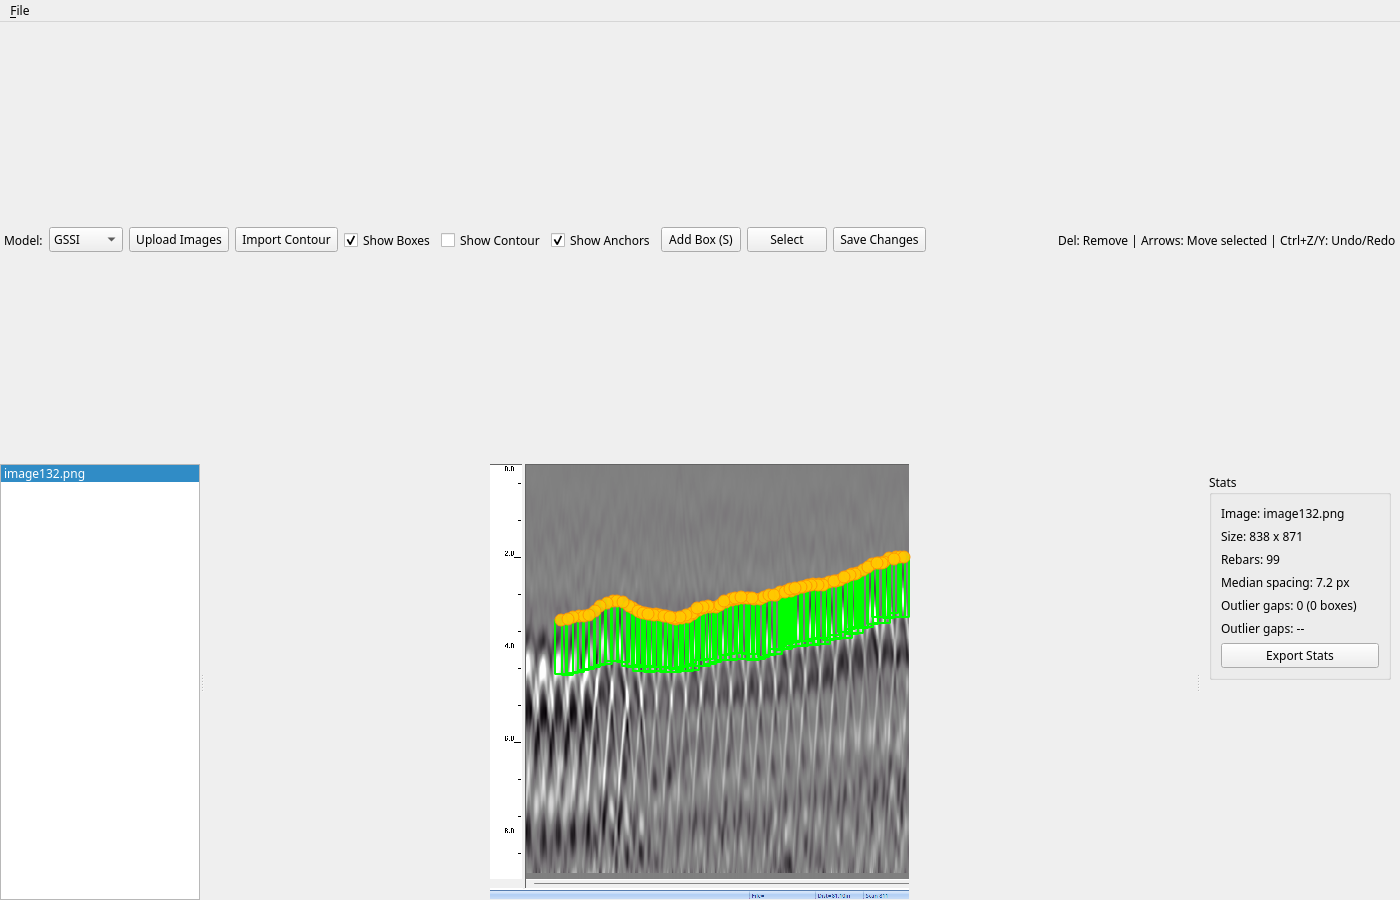
\includegraphics[width=0.98\textwidth]{app/13_gssi_window.png}
% \end{frame}

\begin{frame}{Multi-Image Project}
  \centering
  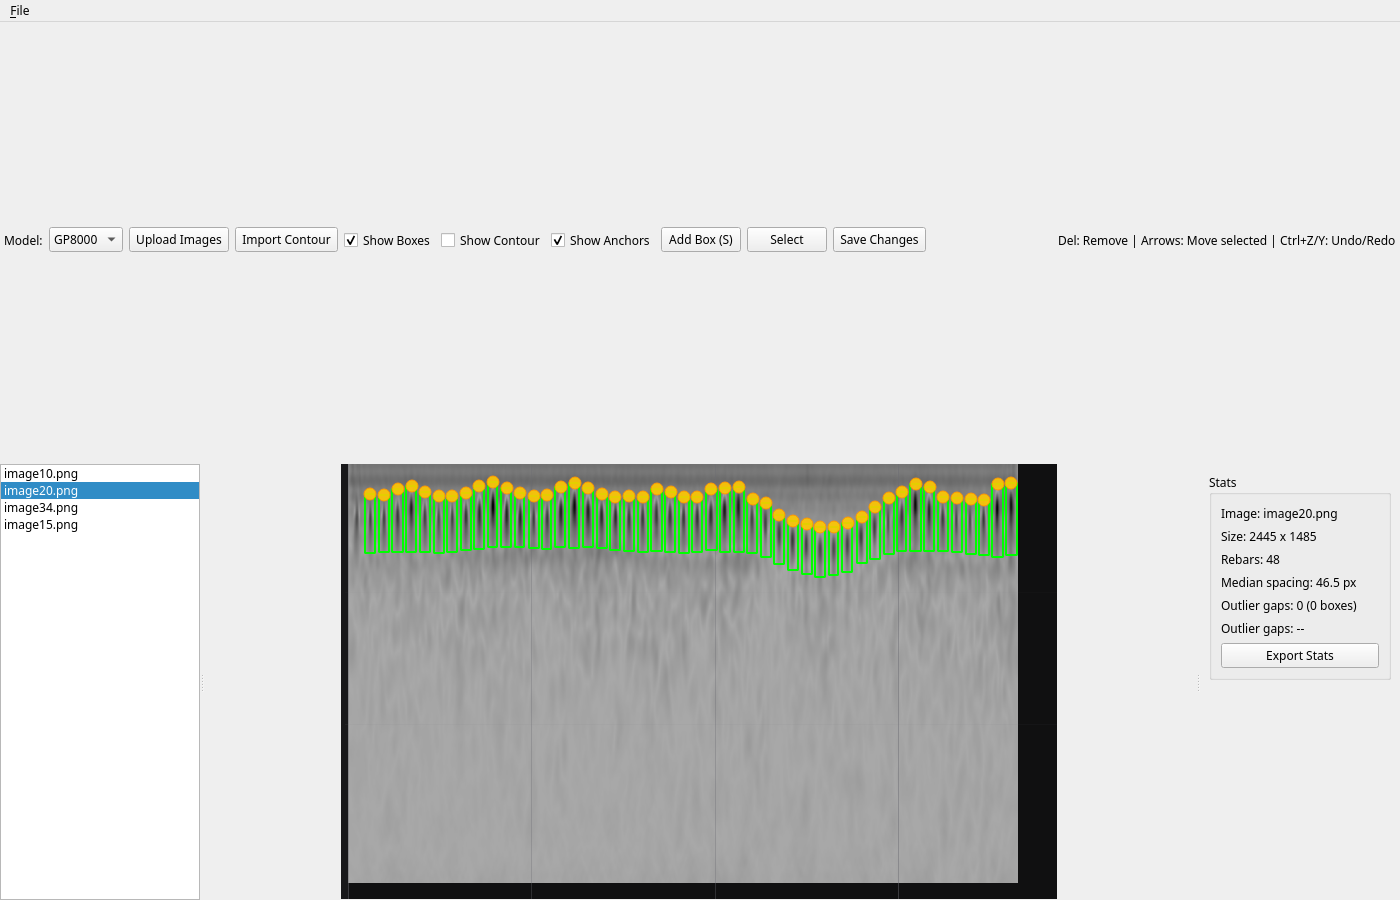
\includegraphics[width=0.98\textwidth]{app/15_multi_image.png}\\[0.3em]
  {\footnotesize\color{mutedtext}Queue many B-scans; per-image boxes and anchors persist}
\end{frame}

\begin{frame}{Human-in-the-Loop}
  \centering
  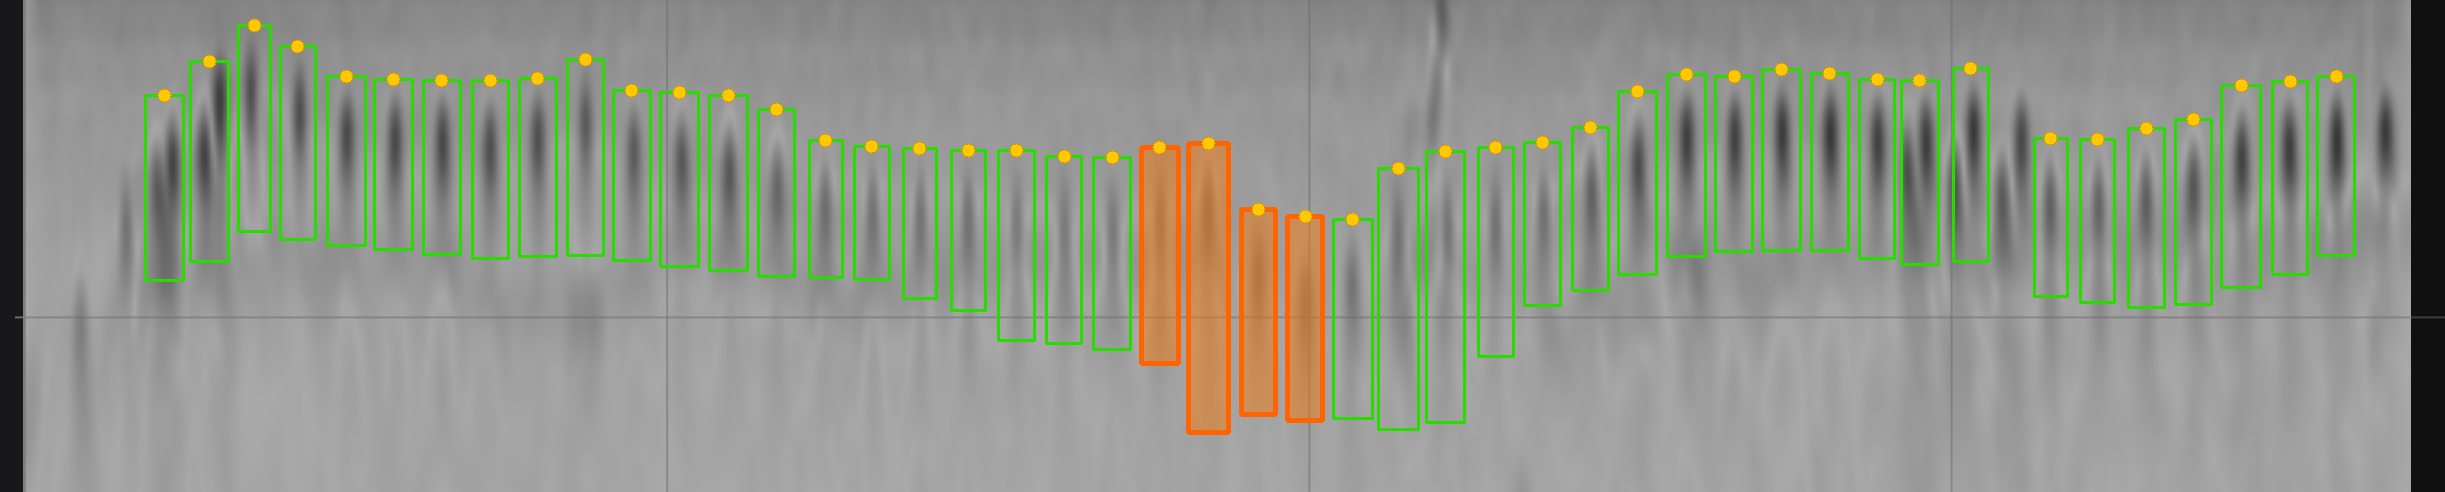
\includegraphics[width=0.95\textwidth]{app/hitl_select_highlight.png}\\[0.2em]
  {\footnotesize\textbf{Select \& delete} --- drag-rectangle across boxes, Del removes them}\\[0.7em]
  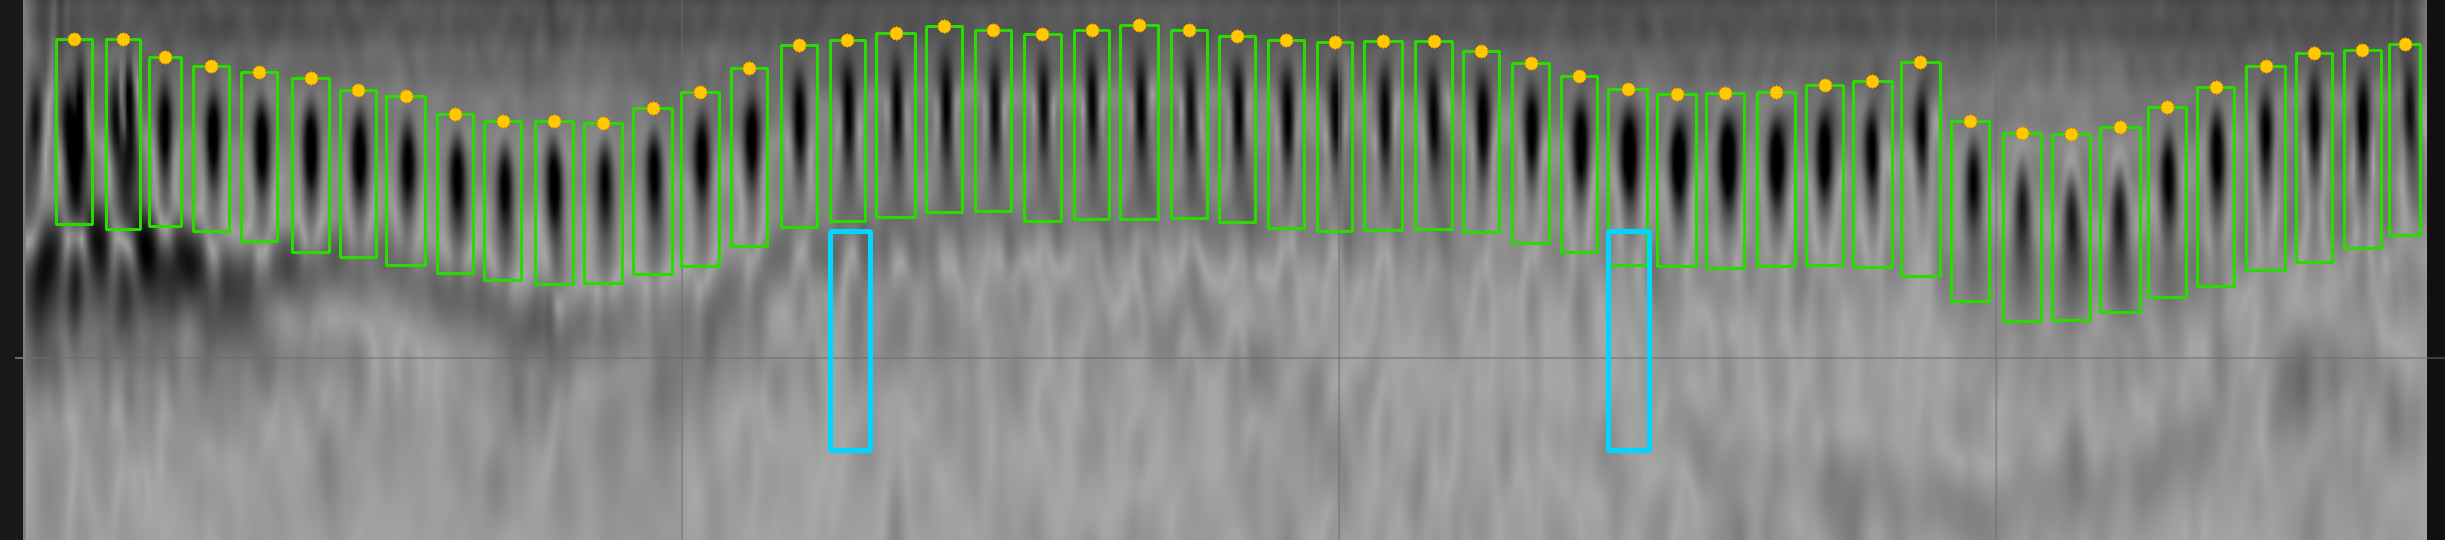
\includegraphics[width=0.95\textwidth]{app/hitl_add_boxes.png}\\[0.2em]
  {\footnotesize\textbf{Add new boxes} --- two clicks in Add mode place a new rebar}
\end{frame}

\begin{frame}{Deformity Classification}
  \centering
  {\normalsize
    $\displaystyle
      \tilde d = \mathrm{median}(d_i) \qquad
      \sigma = \mathrm{std}(d_i) \qquad
      \text{flag if } \lvert d_i - \tilde d \rvert > \max(2\sigma,\; 6\,\text{px})
    $
  }\\[0.5em]
  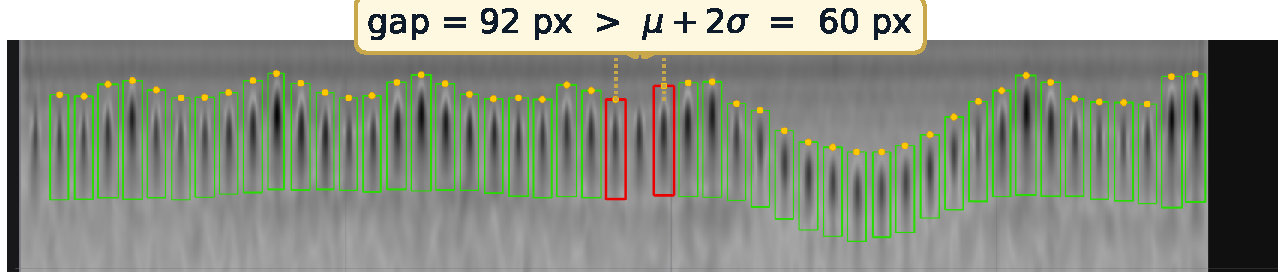
\includegraphics[width=0.98\textwidth]{app/deformity_example.pdf}\\[0.3em]
  {\footnotesize\color{mutedtext}Delete one detection $\to$ the gap between its neighbours exceeds $\tilde d + 2\sigma$ $\to$ both flanking boxes flagged red}
\end{frame}

% ═════════════════════════════════════════════════════════════════════════════
% FUTURE WORK
% ═════════════════════════════════════════════════════════════════════════════
\begin{frame}[plain]
  \vspace{2.8cm}\centering
  {\Huge\color{navydark}\textbf{Future Work}}\\[0.5em]
  {\color{navymid} Defect detection, autonomous carts, collaborators}
\end{frame}

\begin{frame}{Defect Detection}
  \centering
  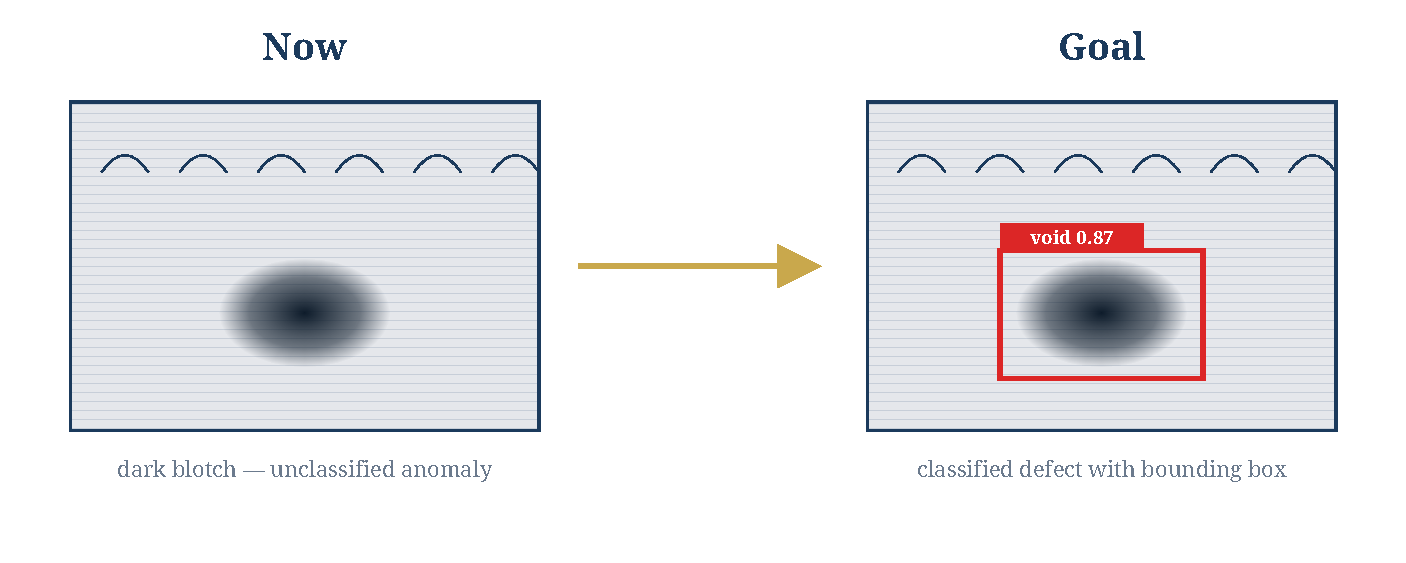
\includegraphics[width=0.92\textwidth]{future/blotch_recognition.pdf}\\[0.4em]
  {\footnotesize\color{mutedtext}From unclassified blotches to labeled defect boxes}
\end{frame}

\begin{frame}{Synthetic Defect Embedding}
  \centering
  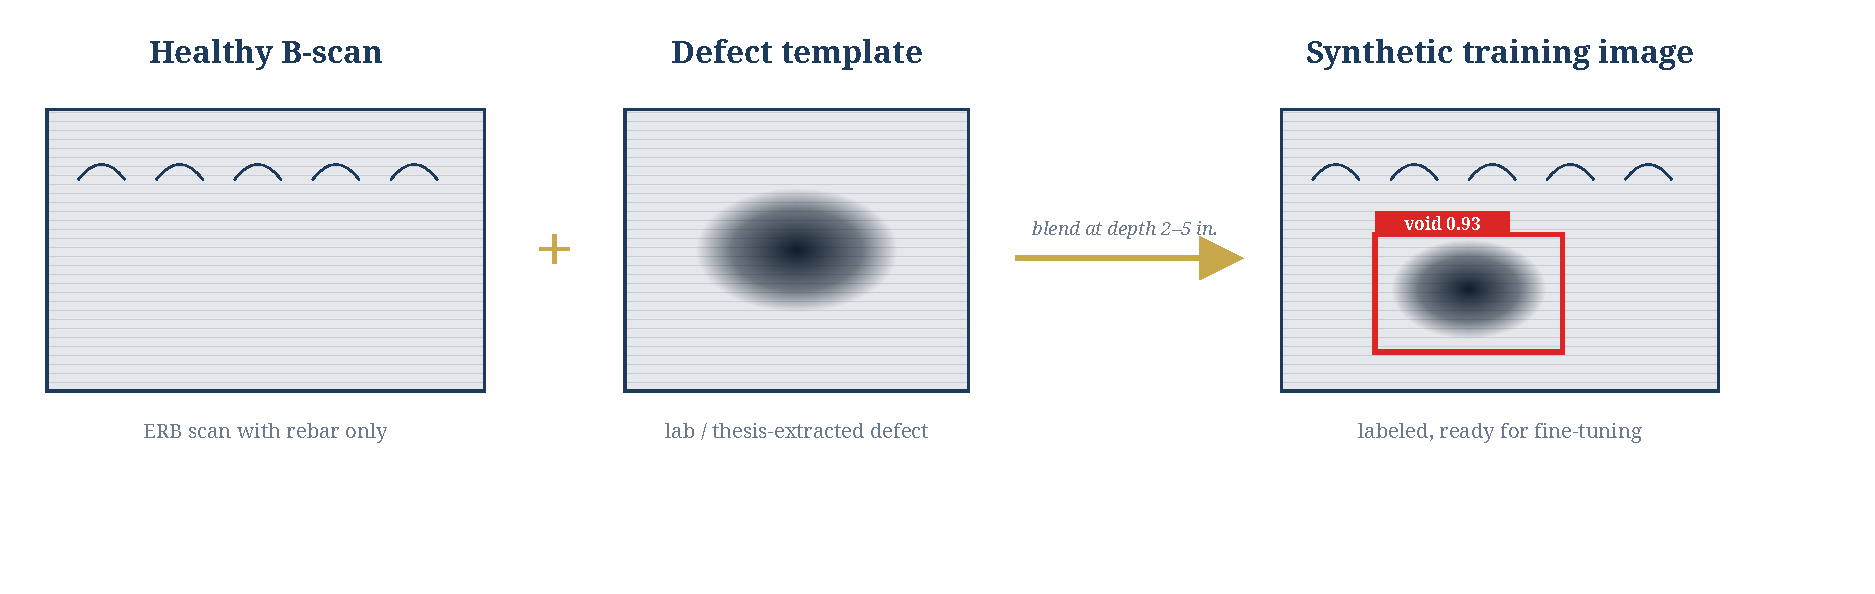
\includegraphics[width=0.98\textwidth]{future/synthetic_embedding.pdf}\\[0.4em]
  {\footnotesize\color{mutedtext}Blend lab defect templates into healthy scans to generate labeled training data}
\end{frame}

\begin{frame}{Autonomous GPR Robotics Augmented Reality}
  \centering
  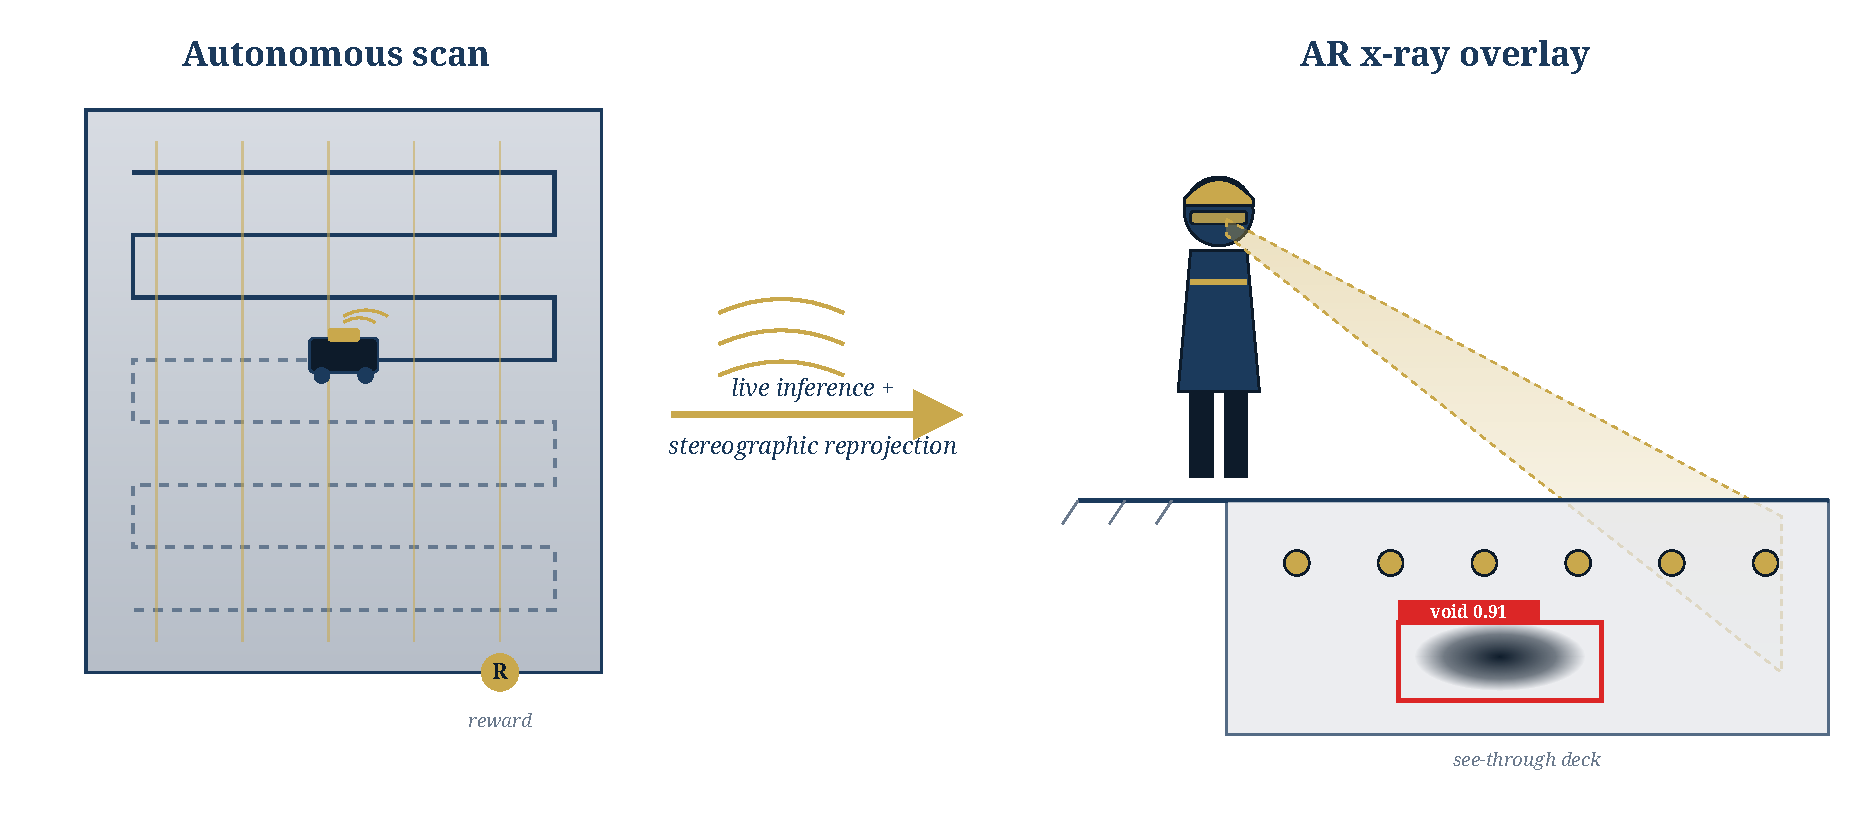
\includegraphics[width=0.98\textwidth,height=0.82\textheight,keepaspectratio]{future/robot_ar.pdf}
\end{frame}

\begin{frame}{Potential Collaborators}
  \centering
  \vspace{1em}
  {\color{navymid}\textbf{Georgia Department of Transportation}}\\[0.4em]
  {\color{navymid}\textbf{Marietta NDT}}\\[0.7em]
  {\large\color{gold}\textit{\ldots and hopefully, you!}}\\[1.2em]
  {\footnotesize\color{mutedtext}Field B-scans from aging bridges \textbullet\ multi-class defect annotation}
\end{frame}

% ═════════════════════════════════════════════════════════════════════════════
% CLOSE
% ═════════════════════════════════════════════════════════════════════════════
\begin{frame}[plain]
  \vspace{1.2cm}
  \centering
  {\LARGE\color{navydark}\textbf{Thank you}}\\[1.2em]

  {\color{navymid} Anish Goyal \textbullet\ Julieta Sanchez \textbullet\ Dr.\ Hossein Taheri}\\[0.4em]
  {\small\color{mutedtext} \texttt{ag29340@georgiasouthern.edu}}\\
  {\small\color{mutedtext} \texttt{js68419@georgiasouthern.edu}}\\
  {\small\color{mutedtext} \texttt{github.com/anishgoyal1108/ConcreteNet}}\\[1.2em]

  {\centering\raisebox{0.4cm}{
\includegraphics[height=1.2cm]{misc/Georgia_Southern_University_Logo.png}}\hspace{1.2em}
\includegraphics[height=2cm]{misc/image1.png}\par}
\end{frame}

\end{document}
